% TEMPLATE for Usenix papers, specifically to meet requirements of
%  USENIX '05
% originally a template for producing IEEE-format articles using LaTeX.
%   written by Matthew Ward, CS Department, Worcester Polytechnic Institute.
% adapted by David Beazley for his excellent SWIG paper in Proceedings,
%   Tcl 96
% turned into a smartass generic template by De Clarke, with thanks to
%   both the above pioneers
% use at your own risk.  Complaints to /dev/null.
% make it two column with no page numbering, default is 10 point

% Munged by Fred Douglis &lt;douglis@research.att.com&gt; 10/97 to separate
% the .sty file from the LaTeX source template, so that people can
% more easily include the .sty file into an existing document.  Also
% changed to more closely follow the style guidelines as represented
% by the Word sample file. 

% Note that since 2010, USENIX does not require endnotes. If you want
% foot of page notes, don't include the endnotes package in the 
% usepackage command, below.

% This version uses the latex2e styles, not the very ancient 2.09 stuff.
%\documentclass[letterpaper,twocolumn,10pt]{article}
%\usepackage{usenix,epsfig,endnotes}

%\documentclass[preprint,nocopyrightspace]{sigplanconf-eurosys}
%\documentclass[letterpaper,twocolumn,10pt]{article}

%\documentclass[10pt,twocolumn,conference]{IEEEtran}

\documentclass[pageno]{jpaper}
\newcommand{\asplossubmissionnumber}{211}

\usepackage[normalem]{ulem}
\usepackage{epsfig,endnotes}
\usepackage{kotex}
\usepackage{subfig}
\usepackage{comment}
\PassOptionsToPackage{hyphens}{url}
\usepackage[hyphens]{url}
%\usepackage{authblk}
\usepackage{hyperref}
\hypersetup{hidelinks}
%\hypersetup{colorlinks=false, citebordercolor={1 1 1}}
\usepackage{multirow}
\usepackage{amsmath}
\usepackage{wasysym}
\usepackage{stmaryrd}
\usepackage{color}
\newenvironment{translatedtext}[2]
   {{\bfseries \color{blue} #1} 
    {\bfseries \color{red}  #2}}

\usepackage{cleveref}
\crefname{section}{§}{§§}
\Crefname{section}{§}{§§}

\usepackage{listings}
\lstset{numbers=left, numbersep=5pt, language=C, xleftmargin=12pt}
\usepackage{algorithm}
\usepackage{algorithmicx}
\usepackage{algpseudocode}

%\hyphenation{op-tical net-works semi-conduc-tor}

\begin{document}

%don't want date printed
%\date{}

%make title bold and 14 pt font (Latex default is non-bold, 16 pt)
\title{OrcFS: Orchestrated File system for Flash Storage} 

%\author[1]{Jinsoo Yoo}
%\author[1]{Joontaek Oh}
%\author[1]{Seongjin Lee}
%\author[1]{Youjip Won}
%\author[2]{Jin-Yong Ha}
%\author[2]{Jongsung Lee}
%\author[2]{Junseok Shim}
%\affil[1]{Hanyang University}
%\affil[ ]{\{jedisty$|$na94jun$|$insight$|$yjwon\}@hanyang.ac.kr}
%\affil[2]{Samsung Electronics}
%\affil[ ]{\{jy200.ha$|$js0007.lee$|$junseok.shim\}@samsung.com}

\date{}
\maketitle
\thispagestyle{empty}

% Use the following at camera-ready time to suppress page numbers.
% Comment it out when you first submit the paper for review.
%\thispagestyle{empty}

\begin{abstract}
In this work, we develop \emph{OrcFS}, which
vertically integrates the log-structured file system and 
the Flash-based storage device. \emph{OrcFS} effectively addresses
three technical issues which the modern Flash-based storage stack which
consists of the log-structured file system and the Flash Storage
suffers from (i) Compound Garbage 
Collection, (ii) Mapping Table Overhead, and (iii) Waste of
Overprovisioning area.
In OrcFS, the log-structured file system and an SSD are tightly
integrated with each other eliminating all the redundancies between the
layers. 
The file system is responsible for address mapping and segment cleaning
while the SSD is responsible for bad block management. The file system
section size is aligned with the superblock size of an SSD so that
segment cleaning activity of the file system effectively consolidates the
valid blocks in the underlying SSD eliminating the need for an SSD to
run its own garbage collection. We develop Disaggregate Mapping,
Block Patching and Quasi-preemptive segment cleaning so that the
log-structured file system is seamlessly integrated with the Flash-based
storage. 
The contribution of OrcFS can be summarized as follows. OrcFS (i) removes 
the root cause for compound garbage collection, (ii)
reduces the mapping table size to 1/54 which eliminates the need for
nearly all DRAM from SSD and (iii) removes the overprovisioning area
from the SSD. 
We prototyped  OrcFS using F2FS and commodity SSD, Samsung 843Tn with
modified firmware. OrcFS reduces the write amplification by 26$\%$ and
increases random write IOPS by 45$\%$. 

\end{abstract}

\begin{comment}
In this work, we develop a new IO stack, \emph{OrcFS}, which vertically integrates the log-structured file system and
the Flash-based storage device. The file system and Flash-based storage
have evolved in their own way to optimize itself against the other.
The Flash storage adopts sophisticated software layer called Flash
translation layer to hide its append-only nature from the in-place
update based file system. The log-structured file system has been
proposed to relieve a Flash storage from expensive address translation
and the garbage collection overhead via maintaining the file system
blocks in append-only manner. Despite their elegance, when they are
combined, the IO stack becomes subject to unacceptable performance
deficiency primarily due to the redundant effort to make the room to
accommodating the newly arriving data in both layers. We call this
phenomenon as \emph{Compound Garbage Collection}.  OrcFS
consists of three key technical ingredients: (i) superblock to
segment static binding where the individual superblocks in SSD are
statically bound to the individual system segments, (ii) Block
Patching in the file system to align the IO size with the Flash page
size, and (iii) Disaggregate Mapping which allows the Flash storage to
maintain a subset of its Flash blocks by itself, not statically bound
to the file system segment.  This static binding bears profound
implications in IO stack design. First, the SSD can dispense with
address translation layer since the file system in OrcFS maintains the
mapping between the file system blocks to the physical Flash
pages. Second, more importantly, the static binding entirely
eliminates the root cause for compound garbage collection since the
segment cleaning activity of the log-structured file system directly
consolidates the valid Flash pages in the Flash storage.

We implement a prototype OrcFS. We use F2FS (Flash
Friendly File System) and Samsung 843Tn SSD as the baseline platform and
modify each of them to form OrcFS. OrcFS reduces the SSD
mapping table size by 1/54. OrcFS effectively eliminates the root cause
for compound garbage collection. Subsequently, compared to F2FS over
commodity Flash storage, the OrcFS reduces the write amplification by
40$\%$ and increases random write performance by 77$\%$.
\end{comment}

\section{Introduction}

Flash based storage device strides its way to main stream storage medium
not only in the mobile device or high performance computing but also in
the server and cloud computing area \cite{enterpriseflash2015berry}. The
fraction of Flash storage sales in the entire storage market has
increased from 6.5\% at 2010 to 31.4\% at 2014. It is expected to grow
beyond 50\% by the end of 2016
\cite{http://biz.chosun.com/site/data/html_dir/2016/08/12/2016081202016.html?main_box},
where most of the growth are from the server sector. The 
\$ per byte ratio of SSD against HDD has also dropped from
6$\times$ at 2012 to 2.8 $\times$ at 2016 \cite{ssdprice}. The rapid proliferation of 
the Flash storage is greatly indebted to the introduction of new
technology such as 3D-NAND \cite{3dnand_samsung} and finer process
\cite{davis2013flash}. 

The SSD gets larger and faster. SSD vendors aggressively adopts internal
parallelism, multi-core controller, massive size DRAM to expedite its
behavior. We examine the DRAM sizes of 184 SSD models manufactured
between 2011 and 2015. Fig.~\ref{fig:dram_size} illustrates the results.
The size of DRAM has increased considerably over the years. About 60$\%$
of SSDs which have manufactured recently have 512 Mbyte and 1 Gbyte of
DRAM. As the SSD gets larger, the size of DRAM in the storage device is
going to increase.
%
\begin{figure}[t]
\begin{center}
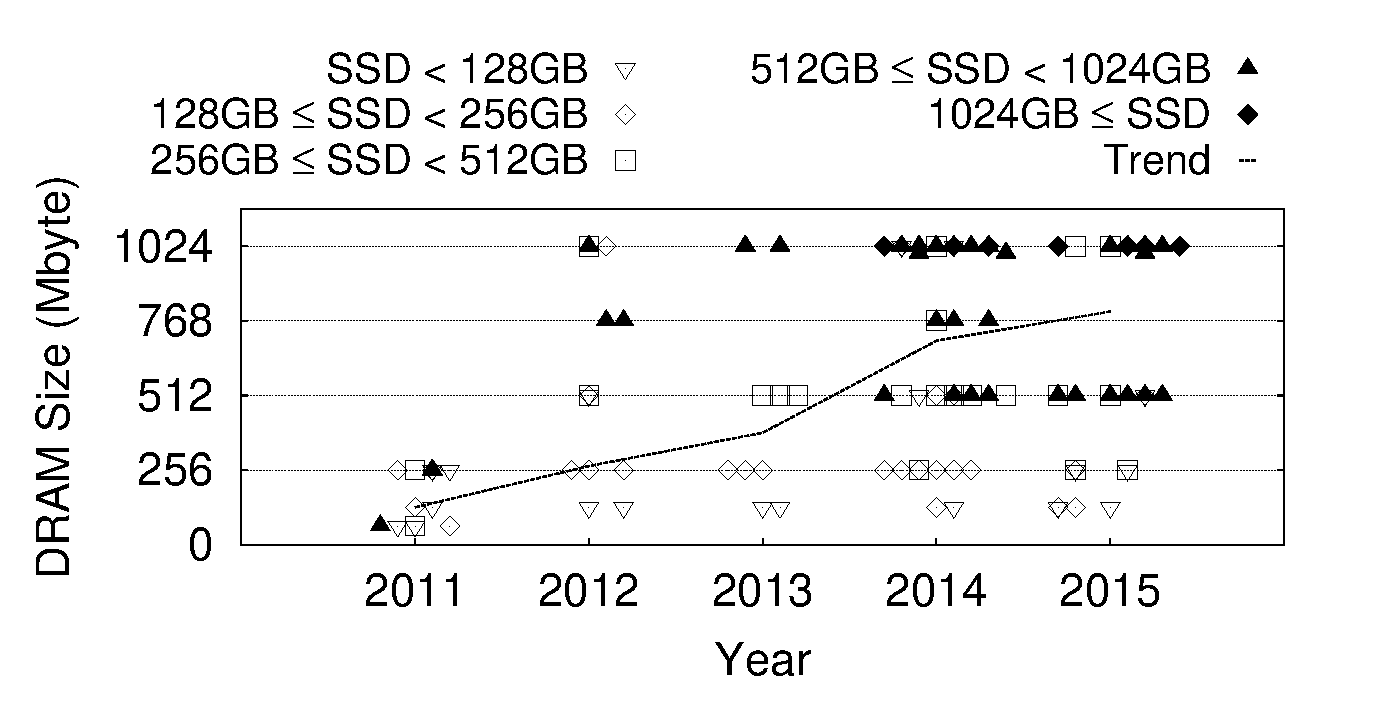
\includegraphics[width=3.6in]{./figure/dram_size.eps}
\caption{DRAM size Trend in SSDs (From 2011 to 2015)}
\label{fig:dram_size}
\end{center}
\end{figure}
%
Despite the sophisticated efforts to harness the SSD with more
horse-power, the host is able to see only less than 50\% of the raw
bandwidth \cite{sdf}. 

The application as well as the filesystem optimize itself to well
exploit the physical nature of the underlying Flash storage. The
application adopts write-optimized and 
append-only search structure such as LSM-tree\cite{FTL for key-value,
chunkstash, SiLK} in its
key-value engine to improve the insert/update operation \cite{Big table,
Cassendra, MongDB, RoksDB}. The filesystems adopts append-only
log structure in managing its filesystem partition \cite{log-structured
filesystem} to align its behavior to the physical nature of the Flash
storage. However, these optimization efforts does not reach far due to
the block device abstraction layer called Flash translation layer
\cite{kim2002space, last08, dftl09, kang2006superblock} in SSD. 
Each of these layers maintains its own mapping table, performs
wear-leveling and garbage collection and reserves a fraction of space
for over-provisioning purpose. The redundancy across the layers brings
significant waste of the storage space and duplicate effort of 
consolidating the valid blocks. The redundancy negatively affect the
storage performance as well as the life-span of the storage device.

This work aims at developing vertically integrated storage stack
eliminating all the redundancies. We develop Orchestrated filesystem,
\texttt{OrcFS} which directly manage the Flash pages. In fact, the
effort to directly manage to Flash storage is not new. It dates back to
more than a decades ago \cite{woodhouse2001jffs, manning2010yaffs} and
the new approaches are still being proposed \cite{nvmkv,sdf,yang2014don,anvil,zhangremoving}. 
While OrcFS shares much of its design philosophy with the preceding
works in that it intends to directly manage the Flash storage \cite{???}, its
actual design uniquely distinguishes itself from the preceding works in
three aspects; First, OrcFS fully eliminates the redundancy in address
mapping via employing Disaggregate Mapping. Second, it fully exploits
internal parallelism of the Flash storage via making the segment
cleaning unit of the filesystem aligned with the superblock size of the
Flash storage. Third, OrcFS adopts Quasi-preemptive segment cleaning to
avoid that the application suffers from excessive segment cleaning
delay. We prototype the OrcFS. OrcFS decreases the memory requirement to
1/56 against page mapping and the write volume by 25\%. The performance
increases by ??? and by ??? against EXT4 under server workload(varmail)
as well as key-value workload(YCSB).  The contributions of
OrcFS are as follows. 

\begin{itemize} 
\item {\bf Reduced Memory Overhead:} OrcFS keeps a large mapping unit yet without the concerns of block thrashing problem. It reduces the size of memory required to store metadata of an SSD by 1/54 of page mapping.

\item {\bf Better Performance:} OrcFS enforces append-only write which guarantees that FTL need not perform in-place update operations. It exhibits 39$\%$ better performance than Ext4 file system. The write amplification in OrcFS is about 26$\%$ lower and IOPS is 45$\%$ higher compared to that of base F2FS in stacked log-structured system. 

\item {\bf Solution to Compound Garbage Collection:} OrcFS resolves compound garbage collection issue inherent in stacked log-structured system. OrcFS sets the unit of segment cleaning same as the unit of garbage collection in the storage device. Since the units on both layers are the same, the storage simply can erase the blocks without any redundant copies and removes the redundant garbage collection overhead between host and the FTL. 
\end{itemize}

The rest of the paper is organized as follows. 
\cref{sec:background} describes how log-structured file system and SSDs
work, and issues stacked log system. \cref{subsec:stack_logs}
defines the notion of compound garbage collection problem and provides
an example to explain the problem. \cref{sec:OrcFS_design} and
\cref{sec:OrcFS_implementation} describes design and
implementation of OrcFS, respectively. 
\cref{sec:experiment} shows the
performance of OrcFS through various experiments and workloads. 
\cref{sec:related_works} describes the related work and 
\cref{sec:conclusion} concludes the paper.


\section{Background}
\label{sec:background}

\subsection{Segment Cleaning in Log-structured File System}

Log-structured file system is write-optimized file system
\cite{rosenblum1992design}. The file system minimizes seek overhead by
clustering the data block and the updated metadata block in proximity.
The file system is written in an append-only manner and all out-of-date
blocks are marked as invalid. The file system maintains in-memory
directory structure to locate the up-to-date version of individual file
system blocks. To minimize the disk traffic, the file system buffers
the updates and flushes them to disk as a single unit either when the
buffer is full or when \texttt{fsync()} is called.  The invalid file
system blocks need to be reclaimed to accommodate the newly incoming
writes. The process is called \emph{segment cleaning}. The segment
cleaning overhead is one of the main reasons which bar the wider
adoption of its technology since it makes the file system under
unexpected long delay\cite{seltzer1995file}.

Append-only nature of the log-structured file system is well aligned with
the update-only nature of the Flash device. A few log-structured
file systems have been proposed specifically for Flash storage
\cite{manning2010yaffs, woodhouse2001jffs, lee2015f2fs}.
However, Flash optimized file systems still operates on top of block 
device abstraction provided by the FTL, and thus, it cannot fully exploit 
the raw performance of the SSD \cite{sdf}.


\subsection{Garbage Collection in Flash Storage}

Garbage collection is a process of reclaiming invalid pages in the
Flash storage \cite{agrawal2008design}. Garbage collection not only interferes with the IO
requests from the host but also shortens the lifespan of the Flash
storage. A fair amount of garbage collection algorithms have been
proposed; Greedy \cite{kawaguchi1995Flash}, EF-Greedy \cite{kwon2007ef}, Cost benefit \cite{rosenblum1992design}, and etc.
Various techniques have been proposed to hide the garbage
collection overhead from the host. They include background garbage
collection \cite{smith2011garbage}, pre-emptive garbage collection \cite{lee2011semi}, and
etc. SSD controller allocates separate hardware thread for garbage
collection so that garbage collection does not interfere with IO request
from the host. 

Host helps FTL minimize garbage collection overhead via TRIM command \cite{shu2007data} and
Multi-stream ID \cite{kang2014multi}. Despite that numerous algorithms have been proposed since the
inception of the Flash storage, the garbage collection is still
problematic \cite{kim2016garbage, zheng2015optimize, huang2015garbage, yang2015optimality, hahn2015collect}.  



\subsection{Stacking the Logs}
\label{subsec:stack_logs}

Log-structured file system in its essence is well aligned with the
append-only nature of the SSD. Sequential IO request originated by
log-structured file system can greatly simplify the address mapping and
the garbage collection overhead of the underlying storage.  Recently, a
number of key-value stores exploit append-only update mechanism to
optimize its behavior towards write operations \cite{lim2011silt, ghemawat2014leveldb}. 
However, the log-structured file system for SSD  entails a number
of redundancies whose result can be disastrous. There exist majorly
three redundancies: (i) garbage collection, (ii) mapping information,
and (iii) overprovisioning area.  Fig.~\ref{fig:layered_log_system}
illustrates an example: a log-structured file system over an SSD. 

First, each layer performs garbage collection on its managing address
space. There exist redundant efforts of log-structured storage device to
garbage collect data. We define Compound Garbage collection as the phenomenon 
where the storage level log system performs garbage collection on 
data blocks which are already segment cleaned by a log-structured 
file system. The Compound Garbage Collection not only degrades the 
IO performance but also shortens the lifespan of the 
Flash storage \cite{yang2014don, lee2016application, zhang2016parafs}.

Second, each layer has to manage its own metadata to keep information
for address mapping, and, as a result, larger memory is required to load
the metadata. As the capacity of SSD increases, the overhead of
maintaining the mapping information at Flash page granularity becomes
more significant. 

Third, each of the log layers needs to reserve a certain fraction of its
space, the overprovisioning area. The log-structured file system (or
SSD) sets aside a certain fraction of its file system space (or storage
space) to host the extra write operations caused by garbage
collection. Overprovisioning is an indispensable waste of the expensive
Flash storage. The total amount of overprovisioning areas for individual log
layers can be very significant. 


\begin{figure}[t]
\begin{center}
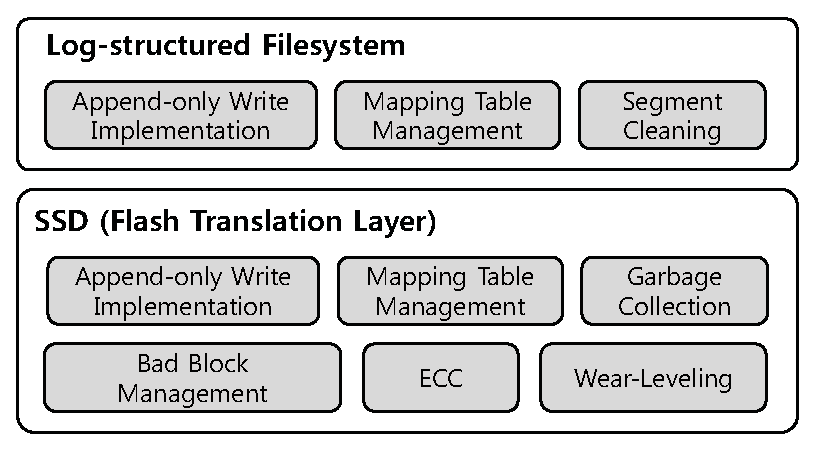
\includegraphics[width=3in]{./figure/layered_log_system}
\caption{Example of Stacking Log System}
\label{fig:layered_log_system}
\end{center}
\end{figure}

\begin{figure}[t]
\begin{center}
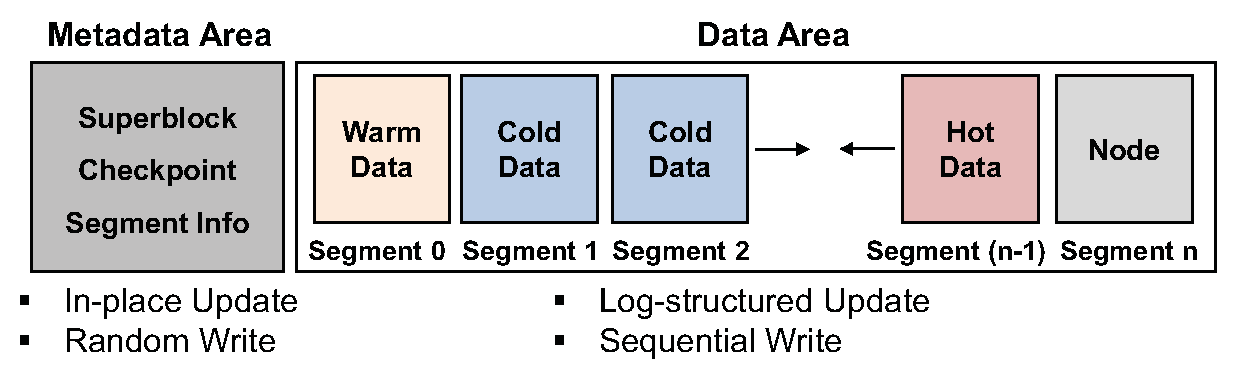
\includegraphics[width=3.4in]{./figure/f2fs_layout}
\caption{F2FS Partition Layout}
\label{fig:f2fs_partition}
\end{center}
\end{figure}


\section{Design: Orchestrated File System}
\label{sec:OrcFS_design}

\begin{comment}
\begin{figure*}[t]
\centering
 \subfloat[Ext4 with Page mapping SSD]{
 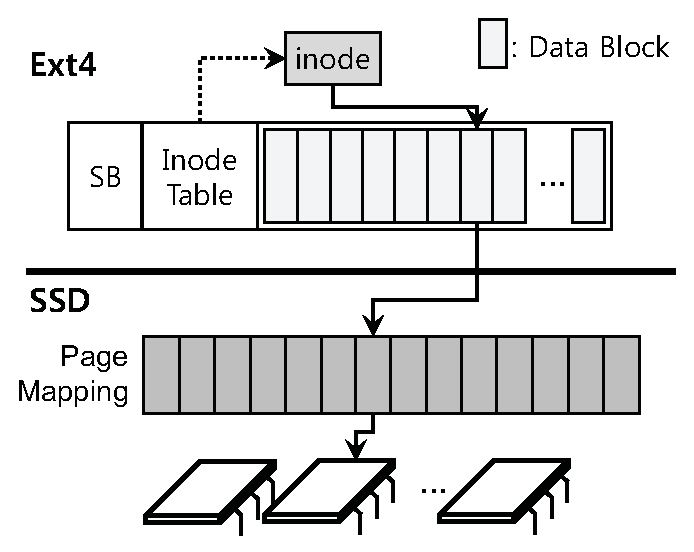
\includegraphics[width=2in]{./figure/ext4_arch}
 \label{fig:ext4_layout}
 }
 \subfloat[F2FS with Page mapping SSD]{
 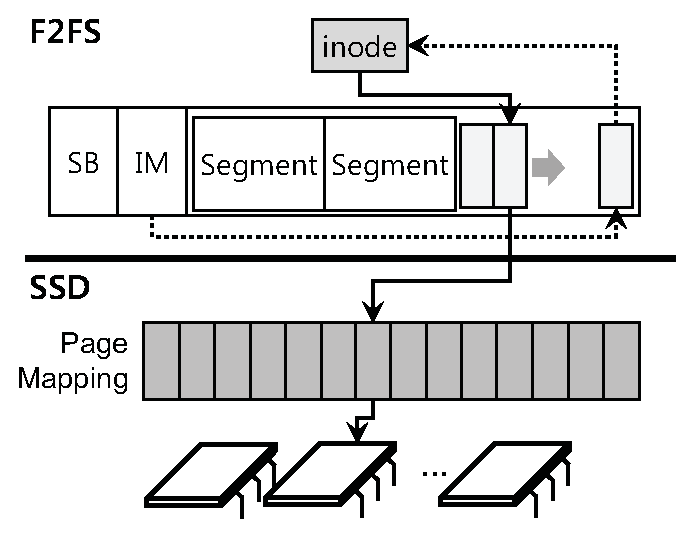
\includegraphics[width=2in]{./figure/f2fs_arch}
 \label{fig:f2fs_layout}
 }
 \subfloat[OrcFS]{
 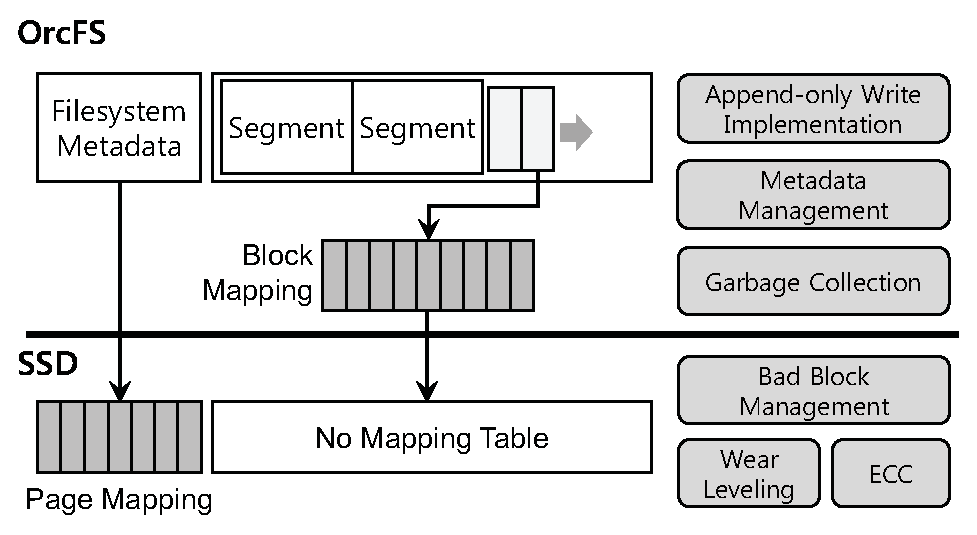
\includegraphics[width=2.06in]{./figure/usl_architecture}
 \label{fig:usl_layout}
 }
\caption{System Layout for Different File Systems and SSD Mapping
  Scheme (SB: Superblock, IM: Inode Map)}
\label{fig:system_layout}
\end{figure*}
\end{comment}

\begin{figure}[t]
\begin{center}
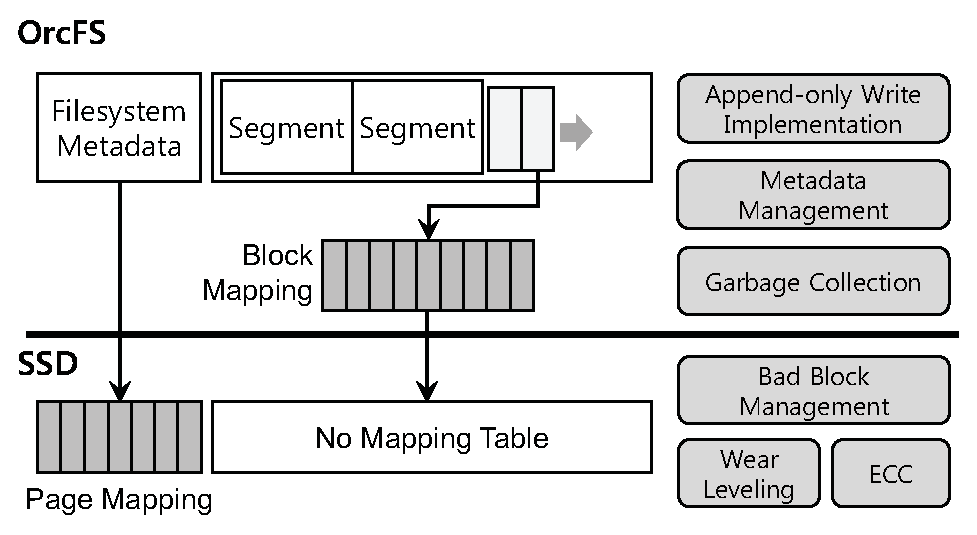
\includegraphics[width=3 in]{./figure/usl_architecture}
\caption{OrcFS Architecture}
\label{fig:usl_layout}
\end{center}
\end{figure}

\subsection{Concept}
In this work, we develop Orchestrated File System, OrcFS, which aims at all 
data structural and operational redundancies across the filesystem and the 
Flash storage. The address translation resides either on the host or on the 
device and subsequently, the redundant garbage collection and redundant 
overprovisioning are entirely eliminated. 
In OrcFS, SSD exposes its physical blocks to the host and leaves most of 
its FTL functions (address translation and garbage collection) to the host 
filesystem. Since the file system is responsible for consolidating the
valid storage blocks, 
the underlying Flash storage does not have to set aside a certain fraction 
of Flash storage for overprovisioning purposes \cite{smith2013understanding}. 

The objective of this work is to vertically integrate the filesystem and Flash 
storage eliminating all redundancies. Eliminating all redundancies, OrcFS can 
reduce the write amplification, save space for overprovisioning, reduce the memory 
requirement of the Flash storage device. Eventually, it improves the performance 
as well as the life span of the storage device. Also, via reducing the memory 
requirement and eliminating the need for overprovisioning, we can build the Flash 
storage in much less expensive manner.

The first issue is to design a right log-structured filesystem for Flash storage. 
Since the log-structured filesystem first appear \cite{rosenblum1992design}, fair 
amount of log-structured filesystems have been proposed during the past few decades \cite{engel2005logfs, nilfs2006, lee2015f2fs}. While append-only nature of log-structured filesystem ideally well 
fits with the physical characteristics of the Flash storage, most log-structured 
filesystem fail to address the critical issues inherent in log-structured filesystem; 
segment cleaning overhead, \texttt{fsync()} overhead, and inability to handle direct 
IO. Due to this reasons, Few works have gone beyond an academic exercise and are used 
in very specialized environment \cite{nilfs2006}. Recently proposed F2FS \cite{lee2015f2fs} 
well addresses most of the existing issues in log-structured filesystem properly 
exploting the append-only nature and good random write performance of Flash storage.

As a initial design choice, we adopt 
F2FS to manage physical NAND Flash storage. Instead of clustering the data 
and the associated metadata together, F2FS maintains the file system metadata 
and the data in the separate region (Fig. \ref{fig:f2fs_partition}). 
F2FS updates the metadata region 
and the data region in in-place manner and append-only manner, respectively.
For data region, F2FS categorizes the 
data blocks into six categories subject to the file extensions and access 
frequency. This greatly improves the efficiency of consolidating the blocks 
in the log-structured file system via clustering the file blocks with 
respect to their update frequencies. 

In OrcFS, the storage blocks in the underlying Flash storage are partitioned 
into two regions: Page Granularity Partition and Section Granularity Partition. 
Each of these two partition occupies contiguous space in the storage.
The size of 
these partitions is aligned with the section size of the F2FS file system.
F2FS provides a notion of ``Section’’. Section is a set of consecutive filesystem 
segment. Section is a unit of segment cleaning in F2FS. Filesystem segment usually 
corresponds to the NAND Flash block. In F2FS, the size of the segment and the 
section can be adjusted at filesystem format phase. By default, a section consists 
of single segment. In OrcFS, each of these storage partitions is statically bound 
to the metadata region and the data region of the filesystem. Each of the partition 
is statically bound to the metadata region and the data region of the file system. 

Recent efforts to directly manage the Flash storage \cite{zhang2016parafs, lee2016application} 
still retain the mapping information at the Flash storage. The primarily 
focus on transforming an application workload and the associated metadata 
updates into a section aligned sequential append only workload. This enables 
the underlying Flash storage to eliminate expensive page mapping and to 
adopt block mapping instead \cite{qin2010demand}. 

OrcFS entirely eliminate any redundancies in logical to physcial address 
mapping in the Flash storage. For metadata region, OrcFS delegates the address 
translation to the Flash storage. The Flash storage maintains its own mapping 
table for the page granularity partition. Since page granularity partition is 
bound to metadata region of F2FS, OrcFS leaves the management of physical Flash 
blockes for filesystem metadata region to the Flash device. For data region, 
OrcFS is responsible for managing the physical Flash blocks. When the LBA for 
an incoming IO requests is for section granularity region, the Flash storage 
recognize the LBA as a physical address of a flash block and direct the requests 
to the respective location. 
Fig. \ref{fig:usl_layout} illustrates the schematic 
organization of the OrcFS.

The key ingredients of OrcFS are Disaggregate 
Mapping, Quasi Pre-emptive Segment Cleaning. 
We adopt superblock in managing the Flash storage \cite{park2009sub, seong2010hydra}. 
We develop Quasi Pre-emptive Segment Cleaning to minimize the interference 
of the section cleaning against the foreground I/O. Fig. \ref{fig:f2fs_partition}, 
there are two regions in F2FS partition.

\begin{figure}[t]
\begin{center}
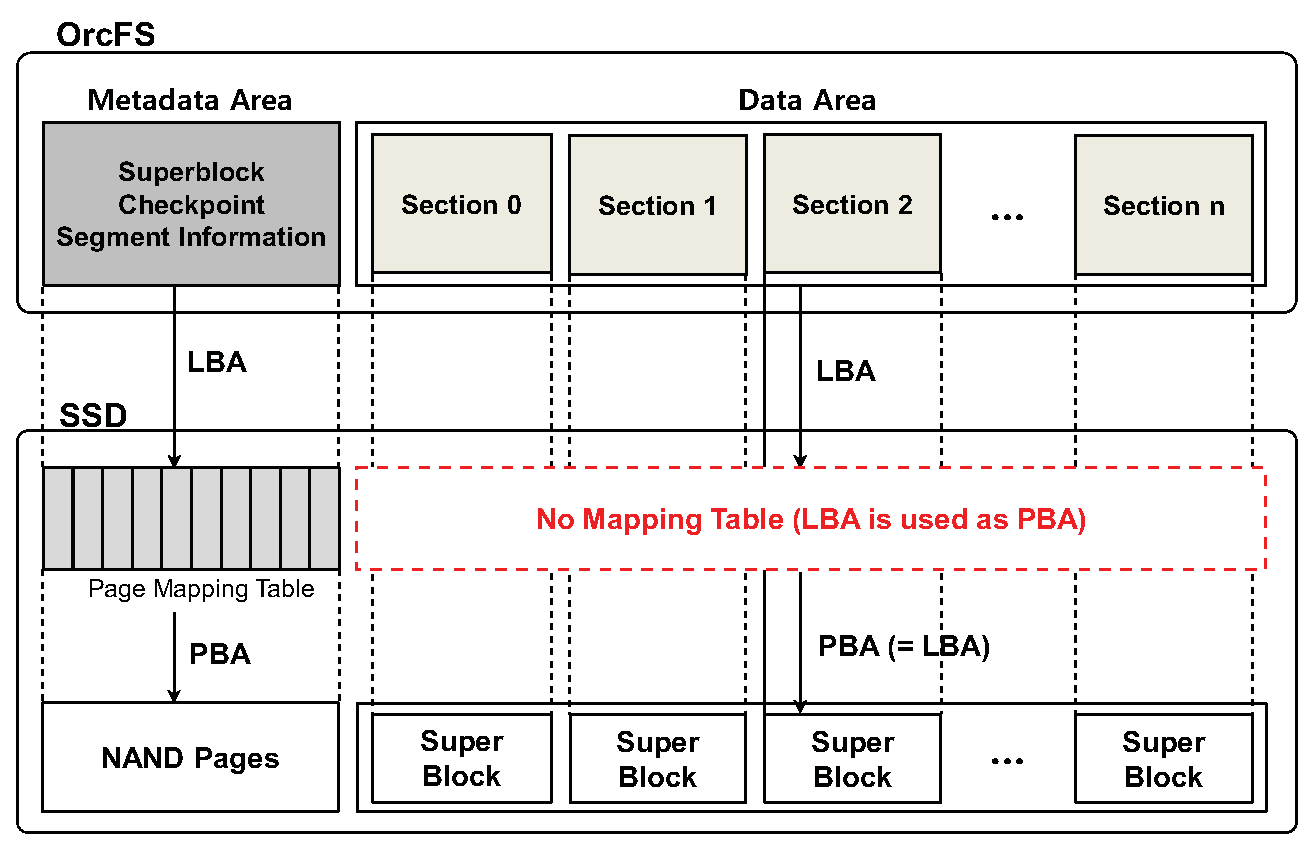
\includegraphics[width=3.2in]{./figure/usl_layout}
\caption{Disaggregate Mapping Layout}
\label{fig:da_mapping_layout}
\end{center}
\end{figure}



\subsection{Disaggregate Mapping}
\label{subsec:da_mapping}

The crux of OrcFS is Disaggregate Mapping. OrcFS manages the two 
file system regions, metadata region and data region, differently,
both vertically and horizontally. 
OrcFS applies different address mapping granularities to each file 
system partitions. It applies page mapping and superblock mapping 
for metadata region and data region, respectively. Different layers 
of the I/O stack manage the two file system partition. As in F2FS, it 
updates the metadata region in-place manner, and delegates the address mapping for 
this region to Flash storage. OrcFS applies append-only updates to 
data region and is responsible for managing it directly. OrcFS 
physically binds the page granularity partition and section granularity 
partition of the Flash storage to metadata region and data region of 
the file system.

The key advantage of OrcFS is superblock unit based storage management. 
Superblock is a set of Flash blocks at the same offset in the Flash chips 
from each channel and from each way \cite{park2009sub, seong2010hydra}. 
Consider 4 channel 2 way SSD. If we assume that a Flash block is 2 Mbyte, 
the superblock consists of eight Flash blocks occupying the same offset 
from each channel and way combination. The superblock size corresponds to 
16 Mbyte in our example
In OrcFS, data region is an array of a fixed size 
sections. The section is a unit of segment cleaning. The file blocks in a 
section are consolidated together, and after consolidation, the entire 
section becomes free. OrcFS establishes the size of a section as the 
size of a superblock. Each filesystem section is statically bound to 
each superblock in the flash storage. This section-based allocation 
enables OrcFS to fully exploit the internal parallelism in the underlying 
Flash storage leveraging the append-only sequential write characteristics 
of the log-structured filesystem.

Superblock-based management is not 
without a challenge: inaccurate block clustering and excessive segment cleaning
overhead. In its original form due to its large size, it is 
more difficult for SSD firmware to form a superblock with the Flash pages 
with similar hotness. In OrcFS, the fileystem is responsible for allocating 
the physical Flash blocks to a given page cache entries. It classifies a 
block bases upon the block type, e.g. data block v.s. directory block, 
filesystem extension, e.g. mp3, mov, and etc. OrcFS clusters file blocks 
together with respect to the category and hotness and therefore achieves 
fairly accurate block clustering \cite{ lee2015f2fs, min2012sfs}. 
The overhead of section cleaning will detail with in the subsequent section. 
By making one to one mapping between a section in OrcFS and a 
superblock in SSD, OrcFS can maximize the channel/way parallelism 
in issuing the write requests on a section. 

The SSD Firmware makes the decision over received LBAs. If they are 
for metadata area, the firmware directs them to page mapping managed 
region of the device; if LBAs is for the section granularity region, 
the firmware recognizes them as PBAs.

OrcFS successfully eliminates the redundancy in address translation. 
Mapping information for metadata area and data area are harbored by 
storage device and the host, respectively. 
For 4 Tbyte SSD, the legacy page mapping requires 
4 Gbyte of DRAM for page mapping table. OrcFS requires only 9 Mbyte
at the storage device for mapping table for metadata region. 
While eliminating the redundancy in address translation 
looks simple and straightforward, it has profound implication on 
the behavior of SSD. It entirely eliminates the possibility of 
compound garbage collection \cite{yang2014don}.

The Flash storage is relieved from the burden of allocating 
surplus storage space (invisible to the host) for consolidating the 
valid blocks. 

In order to guarantee that writes to data area are
sequential, we disabled the threaded logging feature \cite{oh2010optimizations} in OrcFS. 

\subsection{Quasi-Preemptive Segment Cleaning}

\begin{comment}
  \floatname{algorithm}{Pseudocode}
  \begin{algorithm}[tbhp]
  \caption{Function for OrcFS Segment Cleaning}
  \label{pseudo:qpsc}
  \begin{algorithmic}[1]
  \Procedure{OrcFS\_SegmentCleaning}{$N_{Segments}$}
  \State $seg\_no \gets select\_vitcim()$ 
  \For {i$\gets$0 to $N_{SegsPerSec}$}
  \State $segment\_cleaning(seg\_no+i)$ 
  \If{$i \bmod N_{Segments} = 0$}
  \If{b\_io is not empty}
  \State \Return // Preemption
  \EndIf
  \EndIf
  \EndFor
  \EndProcedure
  \end{algorithmic}
  \end{algorithm}
\end{comment}

Log-structured filesystem needs to consolidate the valid filesystem blocks 
occasionally. It is called segment cleaning since it intends to create a free 
segment. In OrcFS, the unit of segment cleaning activity is a section. Due 
to the large size of a section, the application may suffer from excessive 
delay if the I/O which it has issued is interfered with the filesystem 
segment cleaning activity. To address this issue, we develop Quasi-Preemptive 
Segment Cleaning. 

In segment cleaning, segment cleaning module selects victim section and 
copies the valid filesystem blocks in the victim section to the destination 
section. Then, the segment cleaning module marks the victim section as free. 
After then, the segment cleaning module sends the TRIM command \cite{shu2007data} 
with the list of cleaned block numbers as the parameter. The Flash storage 
invalidates and erases the associated Flash blocks later in the time line.

The latency of segment cleaning can be very large. Consider 8 channel 4 way 
SSD with 2 Mbyte block size. The section size corresponds to 64 Mbyte. Assume 
that half of the file blocks in a section are valid. Then, we need to clean 
two sections to create a new free section. Copying 64 Mbyte amount of filesystem 
blocks entail significant latency. It can block the application for more than 
a few seconds and the consequence can be disastrous (Fig. \ref{fig:non_preemptive}). 
The existing log-structured filesystems are not designed for this large segment 
cleaning unit. While details may vary, the segment cleaning unit establishes 
an exclusive lock on the log until it creates a new segment. The subsequent 
operation on the respective partition is temporarily blocked.

OrcFS triggers a segment cleaning if the free space in the
filesystem becomes less than 5\% of the entire filesystem partition size
(foreground segment cleaning) or if the filesystem becomes idle(
background segment cleaning). At the beginning, the segment cleaning
module establishes \texttt{gc\_mutex} lock. It blocks the other
\texttt{kworker} threads from performing write operations till the lock
is cleared. Then, it selects a victim section. Foreground segment
cleaning uses greedy \cite{kawaguchi1995Flash} scheme and background
segment cleaning uses cost-benefit \cite{rosenblum1992design} scheme in
victim selection. After selecting a victim section, the valid blocks in
the victim section are read into page cache. It is worth noting that
valid blocks read from the victim section are categorized as \emph{cold}
block \cite{F2FS}. They are written to \emph{cold} segment. In foreground
segment cleaning, the valid blocks are immediately written to the
storage creating the new clean segment. For background segment cleaning,
the filesystem continues cleaning the next victim segment. 
Segment cleaning module continues cleaning the sections until the number of
free sections increases by one. Once it acquires one new free section,
the segment cleaning modules flushes the dirty node blocks to the
storage and flushes the filesystem metadata. Finally, it releases the
\texttt{gc\_mutex}. 

\begin{figure}[t]
\centering
 \subfloat[Segment Cleaning]{
 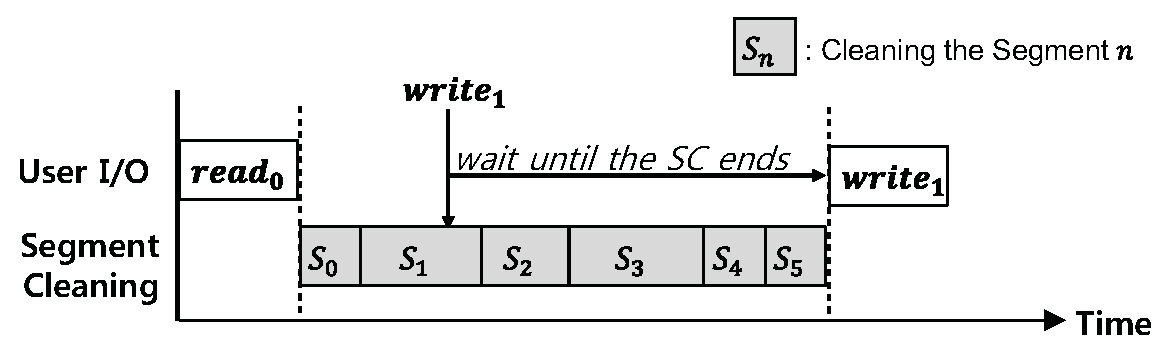
\includegraphics[width=3.4in]{./figure/preemptive_sc_1}
 \label{fig:non_preemptive}
 }\hspace{-1.3em}
 \subfloat[Quasi-Preemptive Segment Cleaning]{
 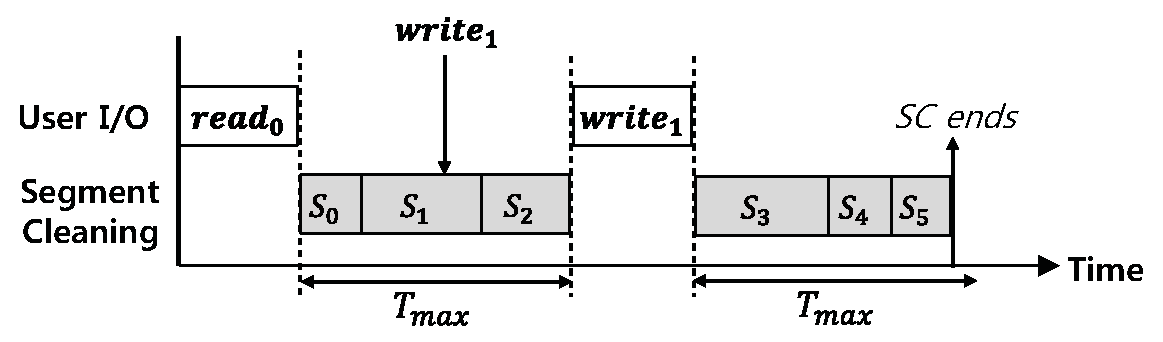
\includegraphics[width=3.4in]{./figure/preemptive_sc_2}
 \label{fig:quasi_preemptive}
 }
 \caption{Different Segment Cleaning Behaviors}
 \label{fig:quasi_sc}
\end{figure}

The \texttt{write()} system call can be interfered with the filesystem
segment cleaning. In servicing \texttt{write()}, the F2FS checks if
there is sufficient free space (5\% free space by default). If there
exist, it allocates a page cache entry for a given \texttt{write()}. If
there is not sufficient free space, the filesystem triggers garbage
collection. Due to this mechanism, even the \texttt{write()}
can be delayed due to the segment cleaning mechanism. The application
which has issued a \texttt{write()} is blocked until the segment
cleaning ends. The delay can be 
prohibitive especially when the segment cleaning unit is large and when
several segments ( or sections in OrcFS ) need to be cleaned due to high
segment (or section) utilization. The \texttt{read()} request is not
blocked by the segment cleaning thread. \texttt{read()} does not require
free block.

To address this problem, we develop Quasi-Preemptive Segment Cleaning,
\emph{QPSC}. We define minimum polling interval, $T_{max}$. When the
segment cleaning starts in OrcFS, it sets the timer to $T_{max}$. After
cleaning each segment, the segment cleaning module examines if the timer
has expired. It continues cleaning the segment if the timer does not
expire. If the timer expires, segment cleaning module examines if there
is any outstanding write() requests. If there exist any pending
\texttt{write()} requests, the segment cleaning module temporarily
releases the lock, \texttt{gc\_mutex()}, and services the pending
requests. After servicing all the pending requests, the segment cleaning
module resumes with the timer reset to $T\_{max}$. If there is not any
pending request, it resets the timer to $T\_{max}$ and keeps cleaning
the segments. Fig.~\ref{fig:quasi_preemptive} illustrates the segment
cleaning in its original form and with Quasi-preemptive feature. 
The VFS layer of Linux OS maintain a list of inodes for which there
exist outstanding write requests:  \texttt{b\_io} field in the
\texttt{bdi\_writeback} structure. The segment cleaning module examines
this list if it is empty. 

To preserve the context of the segment cleaning, we introduce a new kernel
object, \texttt{SC\_context}. \texttt{SC\_context} maintains the victim
section id, the id of the most recently cleaned segment and
\texttt{has\_victim} flag to determine if these values are legitimate. The 
segment cleaning module uses this information to determine if segment
cleaning is being performed or if it is a beginning of the segment
cleaning. When the segment cleaning thread wakes up, it reads
\texttt{has\_victim} field and determines where to start the segment
cleaning.

\begin{table*}[t]
  \begin{center}
  \begin{tabular}{|c|c|c|c|c|c|c|c|} \hline
  						& OrcFS 			& ParaFS\cite{zhang2016parafs}	& AMF\cite{lee2016application} & NVMKV\cite{nvmkv} & ANViL\cite{anvil} & FSDV\cite{zhangremoving} & SDF\cite{sdf}	\\
  						& 	 			& 2016					& 2016 		& 2016		& 2015 			& 2015		  	& 2014			\\ \hline \hline
  Mapping Table (Host) 	& $\Rightcircle$ 	& $\Circle$				& $\Circle$ 	& $\times$ 	& $\times$ 		& $\times$ 		& $\times$ 		\\ \hline
  Mapping Table (Device) 	& $\Leftcircle$ 	& $\Circle$				& $\Circle$	& $\varocircle$ 	& $\varocircle$ 		& $\varocircle$ 		& $\Circle$ 		\\ \hline
  Device Mapping Table Size	& 2.2 MB	 		& 10 MB					& 8 MB 		& 1 GB 		& 1 GB 			& $\leq$ 1 GB 	& 8 MB			\\ \hline
  Garbage Collection		& Host 			& Host 					& Host 		& Host 		& Device 			& Device 			& Host 			\\ \hline
  Legacy Interface  		& $\Circle$ 		& $\Circle$				& $\times$ 	& $\Circle$ 	& $\times$  		& $\times$ 		& $\times$ 		\\ \hline
  Overprovisioning 		& $\triangle$ 	& $\triangle$ 			& $\times$ 	& $\Circle$ 	& $\Circle$ 		& $\Circle$ 		& $\times$ 		\\ \hline
  Application 			& General 		& General					& General 	& KV Store 	& General 		& General 		& KV Store 		\\ \hline
  \end{tabular}
  \end{center}
  \caption{OrcFS and Other Systems (`$\Circle$': medium,
  `$\varocircle$': large, '$\triangle$': small, '$\times$': none,
  Mapping table size is based upon 1 TB SSD with 512 KB Flash block, 4
  KB Page.)} 
  \label{tab:compare_usl}
\end{table*}

\subsection{Bad Block Management and Wear-Leveling}
\label{subsec:bad_block_management}

In OrcFS, the storage device is responsible for bad block management and
wear-leveling. An SSD sets aside a
set of NAND Flash blocks as a spare area \cite{chow2007managing}. There are not
visible to the host. SSD provides a bad block management module with bad block 
indirection table. Bad block indirection table consists of a pair of
$<$physical block number, spare block number$>$. Physical block number
denotes the physical block number of the bad block. The spare block number
is the physical block number of the spare block where the IO request for
the bad block is redirected to. In segment cleaning, all the valid
blocks are consolidated to the newly allocated segment. The replacement
block allocated for the bad block is also migrated to the newly
allocated segment. After the replacement block is copied to the newly
allocated segment, the respective bad block mapping table is reset.
Fig. \ref{fig:bad_block} shows how the bad block management layer in SSD
interacts with segment cleaning.


\begin{figure}[t]
\begin{center}
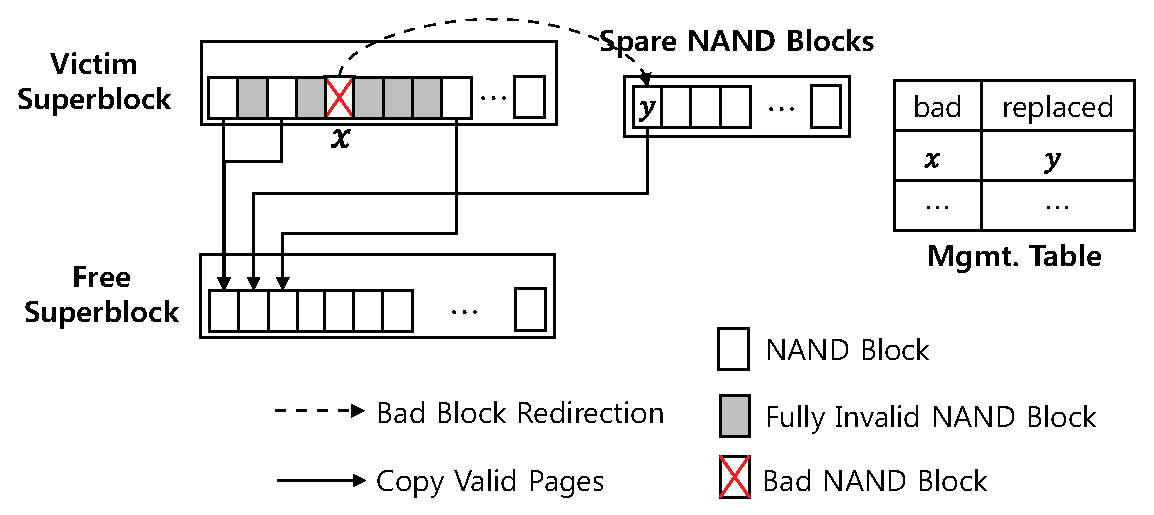
\includegraphics[width=3.3in]{./figure/bad_block_management}
\caption{Segment Cleaning with Bad Block Management}
\label{fig:bad_block}
\end{center}
\end{figure}

There are two approaches in evenly distributing wear of Flash
pages. First, the OrcFS can incorporate the number of wears and selects
the sections with the lowest erase count as the the victim section or as
a destination section. Second, the underlying SSD can introduce simple
mapping table and SSD maps the newly cleaned section to the superblock
with the lowest erase count.

\subsection{Comparison}

We compare the OrcFS with the preceding works in the same category where 
the host directly manages the device to avoid the redundancies across the 
layers. ParaFS \cite{zhang2016parafs} and Application-Managed Flash \cite{lee2016application} 
use F2FS to manage the Flash storage. Both of them propose to use block 
mapping at the device side to exploit the sequential nature of the log-structured 
filesystem. There still exists a redundancy in mapping in these works. 
Both the host filesystem and the storage device introduce the level of indirection.

NVMKV \cite{nvmkv}, ANViL \cite{anvil} and FSDV \cite{zhangremoving} use 
page mapping at the device. ParaFS \cite{zhang2016parafs}, AMF \cite{lee2016application} 
and SDF \cite{sdf} use block mapping. For 1 Tbyte SSD, mapping table size 
corresponds to 1 Gbyte and 8 Mbyte, for page mapping and for block mapping 
respectively. OrcFS requires only 2.2 Mbyte of mapping table at the storage 
device to manage the metadata region. It only requires 1/4 of mapping table 
of the smallest mapping table in the existing works. To use only block mapping, 
AMF modifies the F2FS so that the metadata region is updated in append-only 
manner. While this eliminates the need to manage the metadata region with 
page mapping, it can cause multiple updates in the metadata due to the change 
in the physical location of metadata \cite{rosenblum1992design}. We suspect that this brings non-negligible 
overhead. ParaFS propose to use block mapping (8 Mbyte) and page mapping 
(2 Mbyte) for data region and metadata region. 

Another important aspect is the need to use special interface. It is important 
that the new storage layer is fully functioning without any changes in the 
existing applications and does not need any special interface. Among seven 
works in Table \ref{tab:compare_usl}, only OrcFS, ParaFS and NVMKV are compatible 
with standard API.


The size of the mapping table in FSDV is dynamically resized, 
and in the worst case,
the size of the mapping table becomes the same size as a page mapping table.
NVMKV\cite{nvmkv} removes the host-side metadata and
leverages FTL metadata and interfaces to manage the key-value store.
NVMKV still requires a page granuality mapping table in device.
Also, NVMKV \cite{nvmkv} and SDF \cite{sdf} is limited to a specific
workloads such as key-value store.

ANViL \cite{anvil} lets the host modify device 
logical-to-physical mapping information through a new I/O interfaces, 
but mapping table overhead is still significant.


\begin{comment}
AMF (Application Managed-Flash)\cite{lee2016application} and 
ParaFS\cite{zhang2016parafs} uses log-structured file system in removing 
the overwrite operation in SSDs, and they increased the mapping unit from 
a page to a block. But, the details of each scheme is different.

OrcFS and ParaFS \cite{zhang2016parafs} exploits In-place update in metadata area to avoid ``wandering tree''\cite{rosenblum1992design} problem, and saves metadata using page mapping. The size of page mapping table that manages file system metadata for ParaFS and OrcFS is only 2.2 Mbyte for 1 Tbyte of SSD, which is very small. On the other hand, AMF \cite{lee2016application} takes log-structured approch in managing the file system metadata. Their approach manage all the given partition area with block mapping; however, it must manage in-memory metadata to follow the changes in inode map.
AMF and ParaFS uses the size of NAND block as the unit of the mapping table, but OrcFS uses superblock as the unit. 

ParaFS tries to gather data with the same hotness to a NAND block via 2-D data allocation policy in the file system and NAND block mapping in the SSD. On the other hand, OrcFS allocates data to different sections depending on their hotness. Since each section is mapped to a superblock, write operations in OrcFS can enjoy the maximum parallelism that the device offers without the aid of `Parallelism-Aware Scheduler' proposed by ParaFS. ParaFS warned that the SSDs using superblock as the unit of the mapping may suffer from long garbage collection latency. OrcFS implements quasi-preemptive segment cleaning (QPSC) policy to minimize the host I/O process time while using the section and superblock as the unit of garbage collection. 
\end{comment}

%Another difference OrcFS have compared with AMF and ParaFS is that OrcFS solves block thrashing problem via block patching mechanism. Block thrashing becomes a problem when there is a mismatch in the size of host block, e.g. 4 Kbyte, and the size of page in SSD, e.g 8 Kbyte.


\begin{comment}
A few works proposed that the host holds the
responsibility to manage and modify SSD metadata to improve the
performance of the storage \cite{anvil, nvmkv, sdf}, and reduces the
size of metadata in host or device significantly
\cite{zhangremoving, nvmkv}. Table \ref{tab:compare_usl} shows that
OrcFS has a number of advantages over existing schemes. The size of
the mapping table in OrcFS is small, and unlike FSDV \cite{zhangremoving},
the size is fixed which reduces the management overhead. In OrcFS,
overprovisioning area of an SSD need not be large 
because garbage collection is only performed on a small area for
storing file system metadata. More importantly, OrcFS does not introduce
any new I/O interface to the system; instead, it makes use of
existing ones. Finally, unlike NVMKV \cite{nvmkv} and SDF \cite{sdf}
which targets specific workloads, OrcFS is not limited to a particular
workloads or systems.

Table \ref{tab:compare_usl} summarizes the efforts \cite{zhang2016parafs, lee2016application, anvil, zhangremoving, nvmkv, sdf}.
ANViL \cite{anvil} provides address remapping interface to the host 
system that allows modifying logical-to-physical mapping information
in the device. Since multiple logical addresses can be mapped to a
physical address, it does not require to copy the actual physical
blocks while creating a snapshot, copying data, and in logging a
journal; all it needs to do is remap the logical address. 
FSDV \cite{zhangremoving} modified inodes of a file system to point physical 
addresses of an SSD directly. After updating the inode, the device removes 
the corresponding mapping table entry which allows dynamically reducing 
the SSD mapping table size.
NVMKV \cite{nvmkv} replaced operations for key-value store with FTL 
commands such as atomic multiple-block-write, p-trim, exist, and 
iterate which made it possible to remove in-memory metadata for 
key-value store, and it reduces write amplification considerably.
One other interesting work that improves the performance of Flash-based 
storage is SDF (Software defined Flash) \cite{sdf}. SDF exposes 
the internal Flash channels to the host as an individual block device.
Each channel engine in SDF manages its own block mapping table, bad block management,
and wear-levels of Flash memories. The host system take charge of the garbage collection of the
Flash memory. Thus, the overprovisioning area of SSD is entirely open to
the user.

The work on eliminating the redundancy in file system and SSD firmware is not new in the field; however, they  did not solve the problem entirely. Lee et al. \cite{lee2016application} proposed AMF (Application Managed-Flash) and Zhang et al. \cite{zhang2016parafs} proposed ParaFS that uses log-structured file system in removing the overwrite operation in SSD and increased the mapping unit from a page to a block. In return, the mapping size overhead is reduced to number of blocks from the number of pages in the device. They also provide similar feature that notifies the free space reclaimed during afile system garbage collection to the SSD, so that the SSD does not have to copy data while performing device garbage collection. 

But, the details of each scheme is different. ParaFS \cite{zhang2016parafs} and OrcFS exploits In-place update in metadata area to avoid ``wandering tree''\cite{rosenblum1992design} problem, and saves metadata using page mapping. The size of page mapping table for ParaFS and OrcFS to manage file system metadata is only 2.2 Mbyte for 1 Tbyte of SSD, which is very small. On the other hand, AMF \cite{lee2016application} takes log-structure approch in managing the file system metadata. This approach can manage all the given partition area with block mapping; however, it must manage in-memory metadata to follow the changes in inode map.

AMF and ParaFS uses the size of NAND block as the unit of the mapping table, but OrcFS uses the size of superblock as the unit. ParaFS tries to gather data with the same hotness to a NAND block via having 2-D data allocation policy in the file system and NAND block mapping in the SSD. On the other hand, OrcFS allocates data to different sections depending on their hotness. Since each section is mapped to a supeblock, writes in OrcFS can enjoy the maximum parallelism that the device offers. Unlike ParaFS that has conflict in file system level hotness grouping and parallelism in the SSD, OrcFS does not have such conflict. 

ParaFS warned that the SSDs using superblock as the unit of the mapping may suffer from long garbage collection latency. OrcFS implements quasi-preemptive segment cleaning (QPSC) policy to minimize the host I/O process time while using the section and superblock as the unit of garbage collection. 

Another difference OrcFS have from AMF and ParaFS is that it solves block thrashing problem via block patching mechanism. Block thrashing becomes a problem when there is a mismatch in the size of host block, e.g. 4 Kbyte, and the size of page in SSD, e.g 8 Kbyte. 
\end{comment}

\begin{comment}
  \begin{figure}[b]
  \begin{center}
  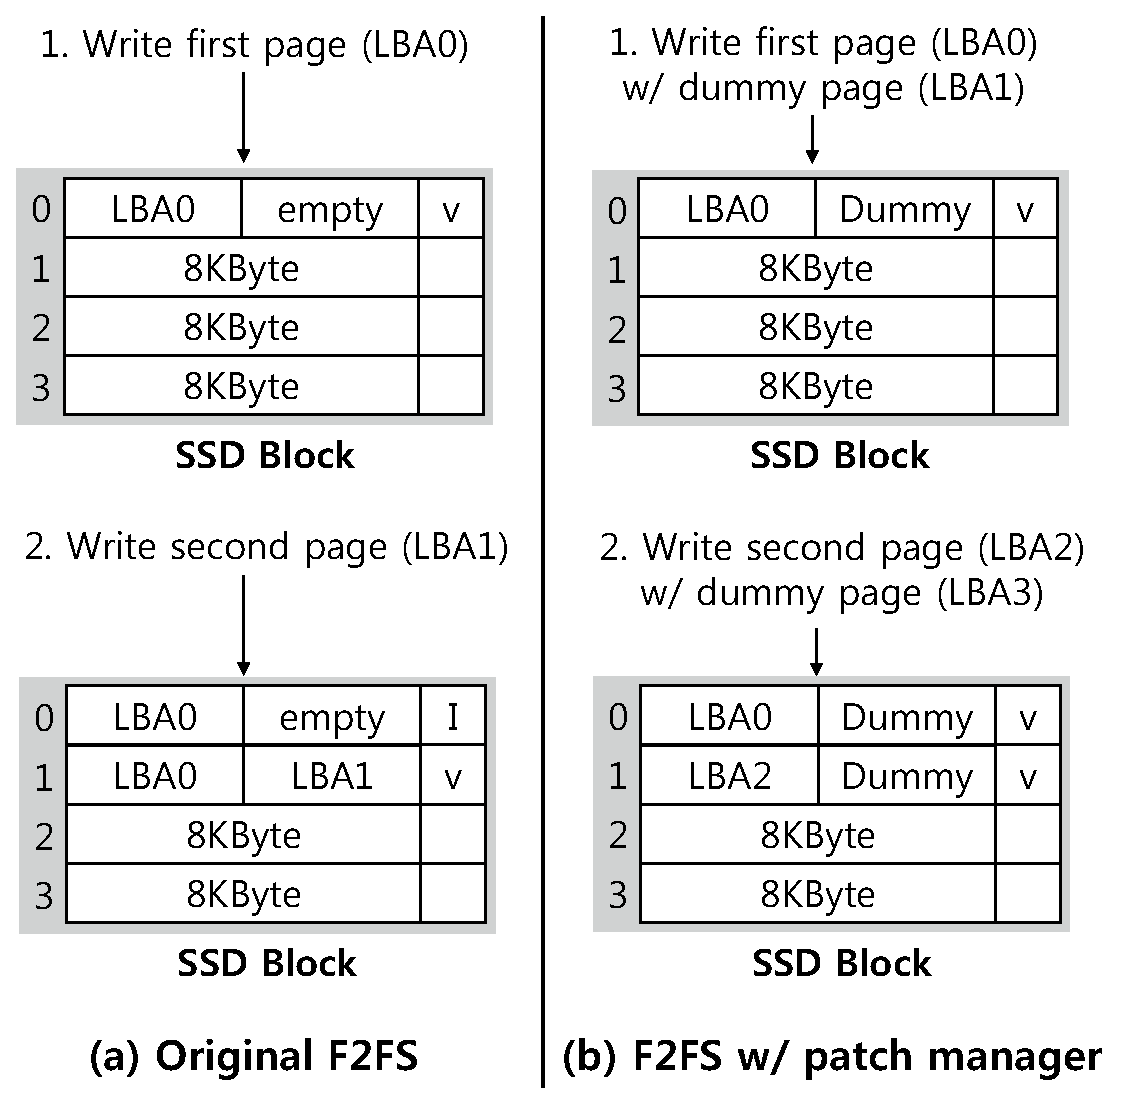
\includegraphics[width=3in]{./figure/patch_manager_ex}
  \caption{Two-page Write Behavior with and without Patch Manager}
  \label{fig:patch_manager_ex}
  \end{center}
  \vspace{-1em}
  \end{figure}
\end{comment}

\subsection{Implementation}
\label{sec:OrcFS_implementation}

\begin{comment}
The file system layer in OrcFS plays two important roles. First, it has
to persistently store the user data in the storage device. Second, it
has to handle garbage collection on data area and send a set of empty
section numbers acquired from segment cleaning process to
storage. Upon receiving the section numbers, the device makes the
corresponding NAND blocks as empty blocks. Therefore, there is no need
to run garbage collection for the NAND blocks belonging to data area but to erase
the target blocks that the file system requested.

Four parts of F2FS is modified to meet the requirements of OrcFS
file system. First, we introduce patch manager to avoid partial writes and second, 
we modified write policy of the file system. Third, we
modified file system formatting tool. Finally, we added a mechanism
to transfer section numbers reclaimed by segment cleaning to OrcFS
storage device.
\end{comment}

File system block size is 4 Kbyte, whereas the page size of an SSD
varies from 4 Kbyte to 16 Kbyte, depending on manufacturers.
In legacy IO stack, SSD
firmware is responsible for handling this discrepancy through request
merge \cite{kim2013partial}, sub-page mapping \cite{qin2011mnftl}, read-modify-write
\cite{agrawal2008design} and etc. In OrcFS, physical Flash page is exposed to
host and the host file system need to take the responsibility of
resolving this misalignment. We develop \emph{Block Patching} for this
purpose.

When the write request size is
not aligned with the NAND Flash page size, OrcFS pads free page cache
entry (4 Kbyte) to the write request to make its size aligned with the
Flash page size. The file system needs to allocate additional file system
block to accommodate the padded page cache entry. While the padded page
cache entry is not reflected in the file size, it consumes an additional
file system block.
The patch manager allocates an
empty page from page cache and concatenates it with original write
request(Fig. \ref{fig:patch_manager}). 
Since a dummy
page does not contain any useful data, we mark it as invalid to let
segment cleaning reclaim the page.

\begin{figure}[t]
\begin{center}
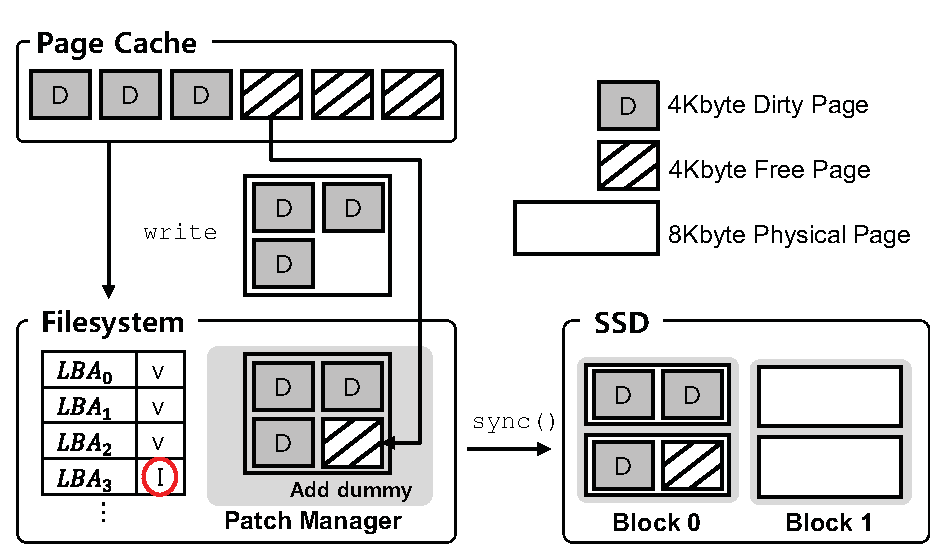
\includegraphics[width=3in]{./figure/patch_manager}
\caption{Block Patch Manager}
\label{fig:patch_manager}
\end{center}
\end{figure}


\begin{comment}
  \begin{figure}[t]
  \begin{center}
  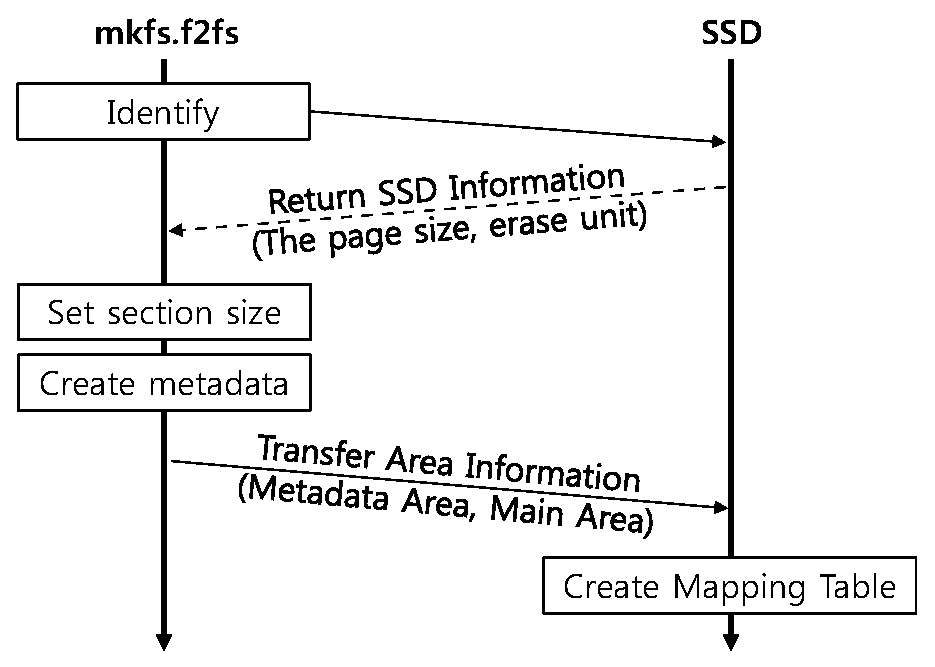
\includegraphics[width=2.5in]{./figure/formatter.eps}
  \caption{Communication between mkfs.f2fs and SSDs}
  \label{fig:formatter}
  \end{center}
  \end{figure}
\end{comment}

\begin{comment}
In order for OrcFS to exploit 
disaggregate mapping scheme, file system needs to understand the page and
block size of the underlying SSD  and the SSD needs to be informed about
the layout of the file system in OrcFS. The negotiation takes in place when
the file system is first formatted on the storage device. 
\end{comment}

In OrcFS, the file system and the storage needs to exchange a few
information; The storage informs the capacity, the Flash page 
size, and the superblock size to the host and the host informs the
storage device about the size of the metadata region. The storage device
uses this information to establish the storage partitions for metadata
region and the data region of the OrcFS filesystem. Currently, we
implement this feature in the filesystem format utility,
\texttt{f2fs\_tools} \cite{f2fs_tools}.

\begin{comment}
  Fig. \ref{fig:formatter} illustrates how mkfs.f2fs and SSD are sharing
  its information. The phase is completed in three steps: (i) In the
  beginning of file system format, OrcFS device acknowledges with its page,
  erase unit, and storage capacity to the file system, (ii) the file system
  sets the  size of a section, creates metadata and data area, and returns
  the area  information to OrcFS storage device, and (iii) the storage
  device  initializes metadata area with page mapping table and let data
  area be  managed by the file system. 
\end{comment}


\begin{comment}
  \begin{figure}[t]
  \begin{center}
  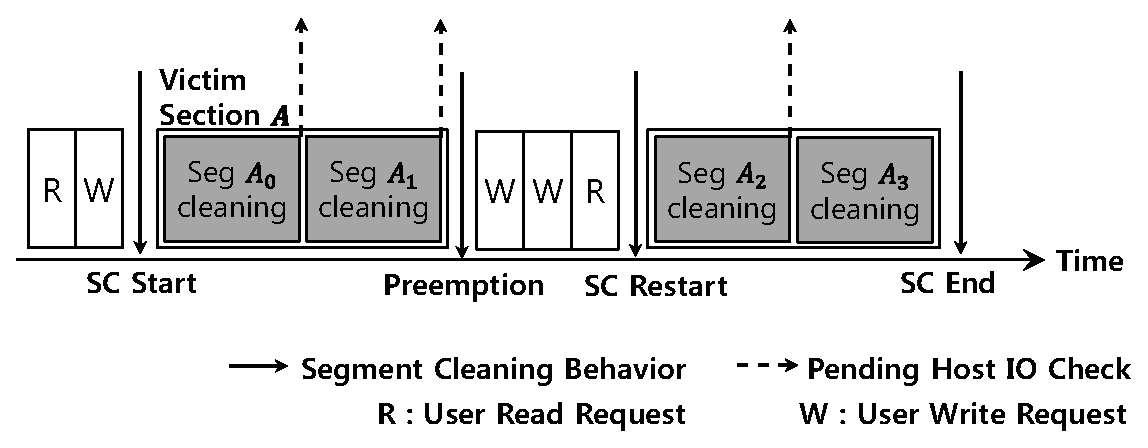
\includegraphics[width=3.2in]{./figure/preemptive_sc}
  \caption{Quasi-Preemptive Segment Cleaning Behavior}
  \label{fig:quasi_sc}
  \end{center}
  \end{figure}
\end{comment}


\section{Experiment}
\label{sec:experiment}

\subsection{Experiment Setup}
\label{subsec:exp_setup}

\begin{comment}
  \begin{table}[h]
  \begin{center}
  \begin{tabular}{|c|c|c|c|} \hline
  		     & F2FS	& Ext4	& OrcFS 		\\ \hline\hline
  File System	& F2FS	& Ext4	& OrcFS	\\ \hline
  SSD Mapping	& Page	& Page	& Disaggregate	\\ \hline
  \end{tabular}
  \end{center}
  \caption{System Information (File System and SSD Mapping Scheme)}
  \label{tab:system_info}
  \end{table}
\end{comment}

We compare the performance of OrcFS against F2FS and Ext4 
on Linux Kernel 3.18.1. OrcFS uses disaggregate
mapping, and F2FS and Ext4 use page mapping SSD. 
We used 
Samsung SSD 843Tn\cite{ssd843tn} for experiments, and modified its
firmware to implement OrcFS. 
To use disaggregate mapping on the device, we disable SSD garbage collection
in the data area, and use the information given by the mkfs.f2fs to bind
the logical address to the physical address. The firmware manages metadata 
area with page mapping table and SSD garbage collection only works for
metadata area.

Table \ref{tab:ssd_info} shows
the specification of the host system and SSD 843Tn used in the performance
evaluations. The SSD performs
garbage collection in units of superblock with the size of 256 Mbyte where
a superblock is a group of NAND blocks with same block number in an array of
Flash memories in channels and ways. 

We set the section size of F2FS to 256 Mbyte in all experiment. 
This is based on the fact that 
the performance is the highest when the size of the section matches 
the garbage collection unit of the storage device. We checked the 
performance of F2FS while varying the size of a section. 
Compared to the IOPS and WAF of F2FS with section size of 2 Mbyte,
F2FS with section size 256 Mbyte shows 24$\%$ higher IOPS and 20$\%$ lower WAF.

We make use of two workloads; 
fileserver, varmail from Filebench\cite{filebench}. Table \ref{tab:filebench}
shows the summary of the each filebench workload.
\emph{fileserver} workload generates 80,000 files with size of 128 KByte, 
then creates 50 threads to issue reads or buffered appends with the ratio of 30:70.
\emph{varmail} creates eight thousand 16Kbyte files using 16 threads to 
create and delete the files with ratio of 50:50, and each operation is 
followed by \texttt{fsync()}.

\begin{table}[t]
\begin{center}
\begin{tabular}{|c|p{3cm}|p{3cm}|} \hline
  		     & Desktop	& Server	\\ \hline\hline
CPU & Intel i7-3770 & Xeon E5-2630 \\ \hline
Mem & 8 GB & 256 GB \\ \hline
OS & \multicolumn{2}{c|}{Ubuntu 14.04 (kernel 3.18.1)} \\ \hline
\multirow{2}{*}{Storage} & \multicolumn{2}{c|}{Capacity: 256 GB (include 23.4 GB OVP)}  \\ 
		 & \multicolumn{2}{c|}{4 MB NAND Block size, 8 KB Page size}  \\ \hline
\end{tabular}
\end{center}
\vspace{-0.7em}
\caption{Host system and Storage (Samsung SSD 843Tn \cite{ssd843tn})}
\label{tab:ssd_info}
\end{table}


\begin{table}[t]
\begin{center}
\begin{tabular}{|c|c|c|c|c|c|} \hline
  		     & Files	& File size & Threads & R/W   & fsync 		\\ \hline\hline
  fileserver	& 80,000	& 128 KB	   & 50	    & 33/67 & N\\ \hline
  varmail 	& 8,000	& 16 KB     & 16	    & 50/50 & Y\\ \hline
\end{tabular}
\end{center}
\vspace{-0.7em}
\caption{Summary of Filebench Workload}
\label{tab:filebench}
\end{table}

\begin{table}[t]
\begin{center}
  \begin{tabular}{|c|r|} \hline 
                         & Mapping Size       \\ \hline\hline 
Page mapping             & 256 Mbyte          \\ \hline 
FSDV \cite{zhangremoving} & $\leq$ 256 Mbyte  	\\ \hline 
Hybrid mapping \cite{last08} & 4 Mbyte \\ \hline 
Disaggregate Mapping     & 1 Mbyte            \\ \hline
\end{tabular}
\end{center}
\vspace{-0.7em}
\caption{Size of Mapping Table (256 Gbyte SSD)}
\label{tab:meta_size}
\end{table}

\subsection{Mapping Table Size}

Table \ref{tab:meta_size} compares the size of mapping tables in 
Page mapping, FSDV \cite{zhangremoving}, Hybrid mapping \cite{last08},
and Disaggregate mapping.
Page mapping uses 256 Mbyte of memory when disaggregate mapping of OrcFS uses
only 1 Mbyte. As the size of SSDs is
increasing, the mapping table overhead becomes significant.
For 1 Tbyte and 4 Tbyte SSD with 4 Kbyte as
the page size, the memory space required to store the mapping table
information is 1 Gbyte and 4 Gbyte, respectively.

File System De-Virtualizer, FSDV \cite{zhangremoving}, makes
file system point to a physical address in an SSD, and the pointed entry
in the SSD is removed from the mapping table. The size of the
mapping table is dynamically resized. In the worst case scenario, it
has to maintain 256 Mbyte of the mapping table, just like the page mapping
table. 

The memory footprint of OrcFS is only 1 Mbyte which consumes
about 256 times less than that of page mapping. Even if we add several
other metadata used by OrcFS, such as segment bitmap and buffered
segment number, the size of total metadata is only 4.73 Mbyte, which
is 54 times less than that of page mapping. LAST FTL consumes is 4 Mbyte
for mapping table.


\begin{figure}[t]
\centering

 \subfloat[Sequential Write]{
 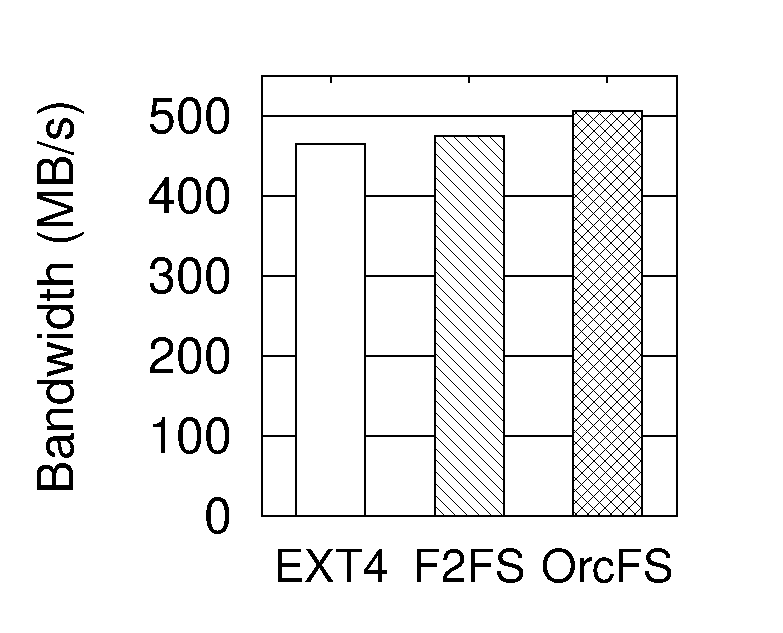
\includegraphics[angle=-90,width=1.55in]{./bench/seq_write}
 \label{fig:benchtest_seqw}
 }\hspace{-1.3em}
 \subfloat[Random Write]{
 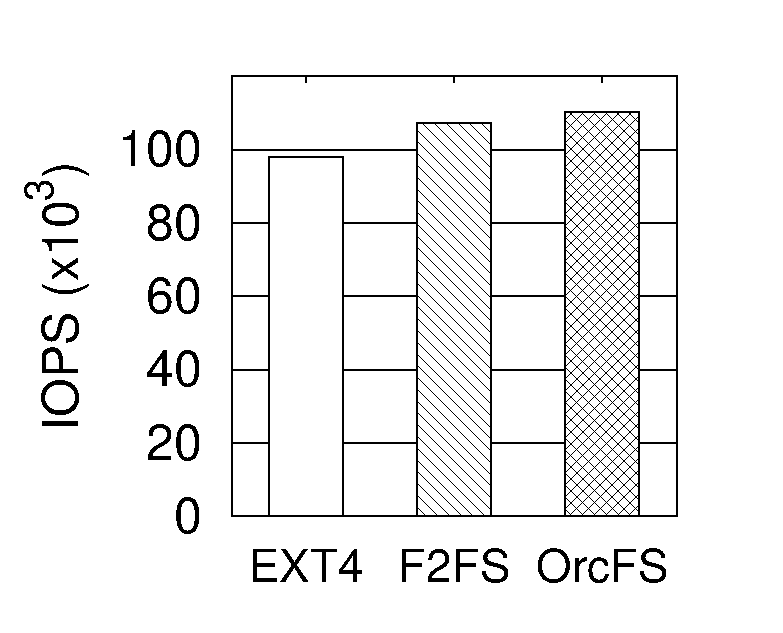
\includegraphics[angle=-90,width=1.55in]{./bench/rand_write}
 \label{fig:benchtest_randw}
 }
 \caption{Sequential / Random Write Performance, F2FS and Ext4 are on
   Page mapping SSD (Workload is as follows. Sequential Write: 188
   Gbyte File size, 512 Kbyte record size, 2.75 Tbyte Total write
   volume / Random Write: 50 Gbyte File size, 4 Kbyte record size, 750
   Gbyte Total write volume, Section size of F2FS: 256 Mbyte)}
 \label{fig:benchtest}
\end{figure}


\subsection{Primitive IO}
\label{subsec:io_performance}


We measure the performance of sequential write and random write (Fig. \ref{fig:benchtest}). 
We format the file system and create a
file with a size of 188 Gbyte. One iteration of an experiment issues 512
Kbyte buffered sequential write until all LBAs are covered and
repeat the iteration for fifteen times.
Fig. \ref{fig:benchtest_seqw} shows the average performance. The
performance of Ext4 and F2FS is 466 Mbyte/sec and 476 Mbyte/sec,
respectively. The performance of OrcFS shows about 507
Mbyte/sec. It is 6$\%$ higher than that of F2FS.

The performance gap between Ext4 and OrcFS stands out more in random 
write workload (Fig. \ref{fig:benchtest_randw}). 
To measure the random performance of
the device, we format the device and create a 50 Gbyte sized file in
the partition. An iteration of the experiment touches all the LBAs
with 4 Kbyte buffered random writes, and the graph shows the average of
fifteen iterations. OrcFS is 12$\%$ faster
than Ext4; IOPS of OrcFS is 110.3 KIOPS and Ext4 is 98.1 KIOPS. 


\begin{figure}[t]
  \begin{center}
  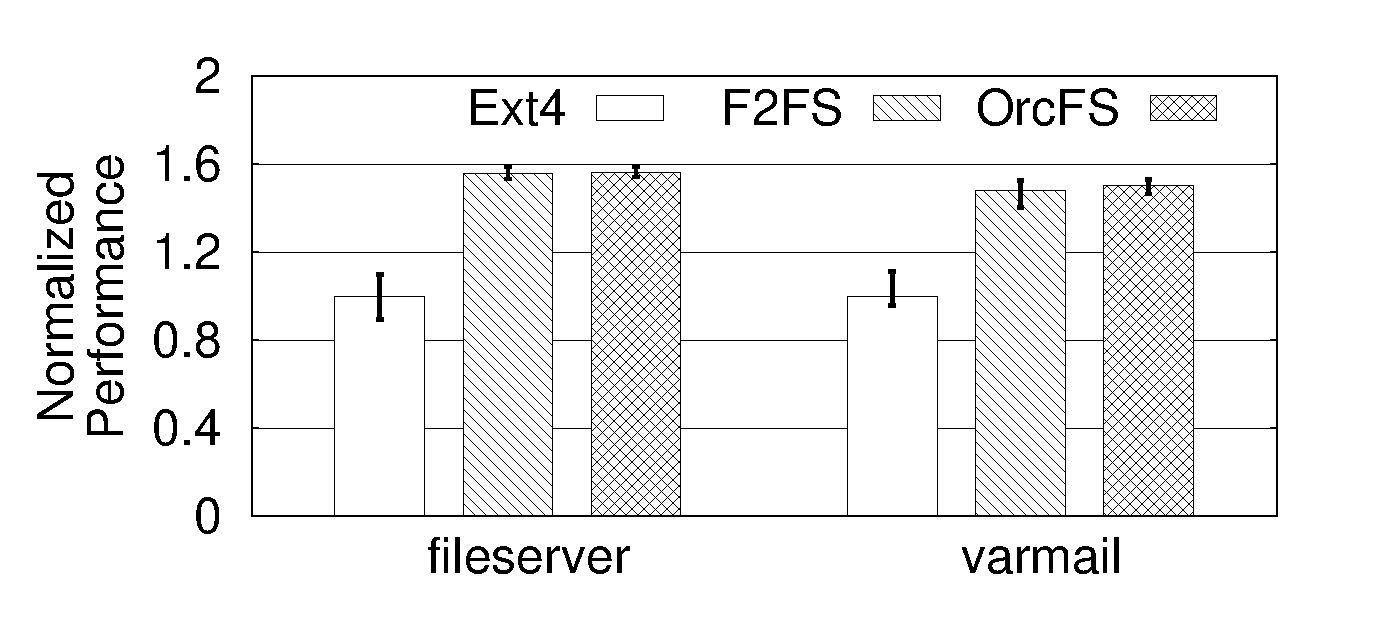
\includegraphics[width=3.2in]{./bench/filebench.eps}
  \caption{Filebench}
  \vspace{-1em}
  \label{fig:filebench}
  \end{center}
\end{figure}

\subsection{Macro Benchmark}
\label{subsec:micro_bench}

{\color{red}
Fig. \ref{fig:filebench} shows the result of filebench \cite{filebench} using \emph{fileserver} and \emph{varmail} workload.  
The performance is normalized with respect to the performance of Ext4. 
In the case of fileserver workload, 
EXT4 shows 225 Mbyte/sec where F2FS and OrcFS exhibit 350 Mbyte/sec and
352 Mbyte/sec, respectively. OrcFS shows 1.6 times better performance
than Ext4. The result is similar in varmail. The performance of OrcFS is
29 Mbyte/sec and Ext4 is 20 Mbyte/sec which is 1.5 times higher.
The performance difference comes from the size of the
blocks passed with \texttt{discard} command \cite{lee2015f2fs}.
Ext4 sends a lot of small sized discard commands but F2FS and OrcFS send
at least segment sized discard commands which significantly reduces the
overhead of processing discard commands in the device.  
}

\subsection{Key-Value Store Workload}
\label{subsec:ycsb_bench}

\begin{comment}
  \begin{figure}[t]
    \begin{center}
    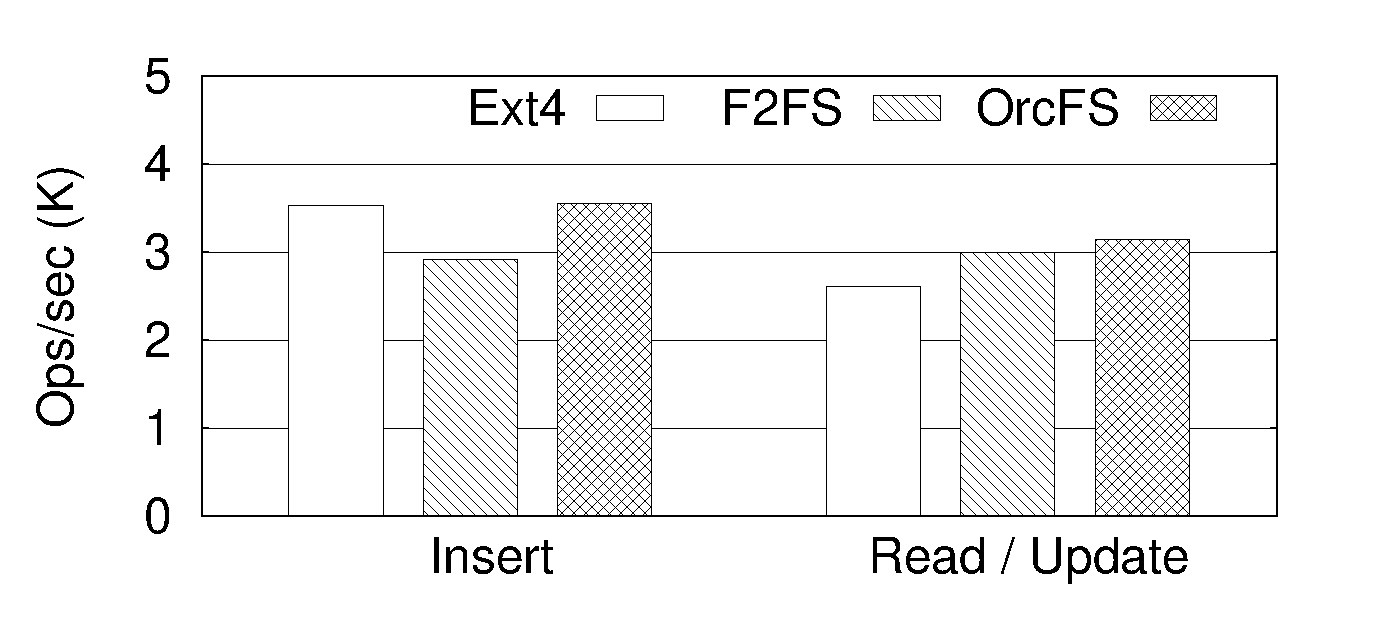
\includegraphics[width=3.2in]{./bench/throughput.eps}
    \vspace{-1em}
    \caption{YCSB Cassandra DB (20 GByte Cassandra DB, 4 KByte Record Size, 50\% read and 50\% Updates; Workload-A)}
    \label{fig:ycsb_throughput}
    \end{center}
  \end{figure}
\end{comment}


\begin{figure}[t]
  \centering
   \subfloat[Throughput]{
   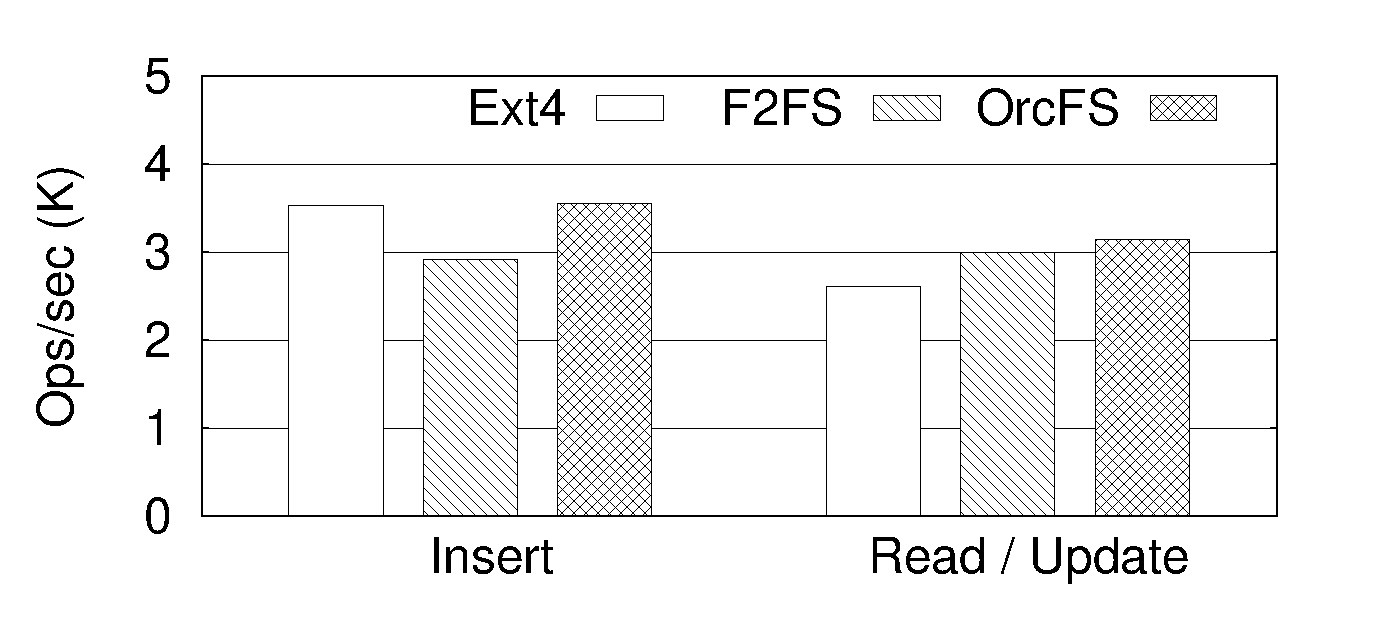
\includegraphics[width=3.2in]{./bench/throughput.eps}
   \label{fig:ycsb_throughput}
   }\quad
   \subfloat[Latency]{
   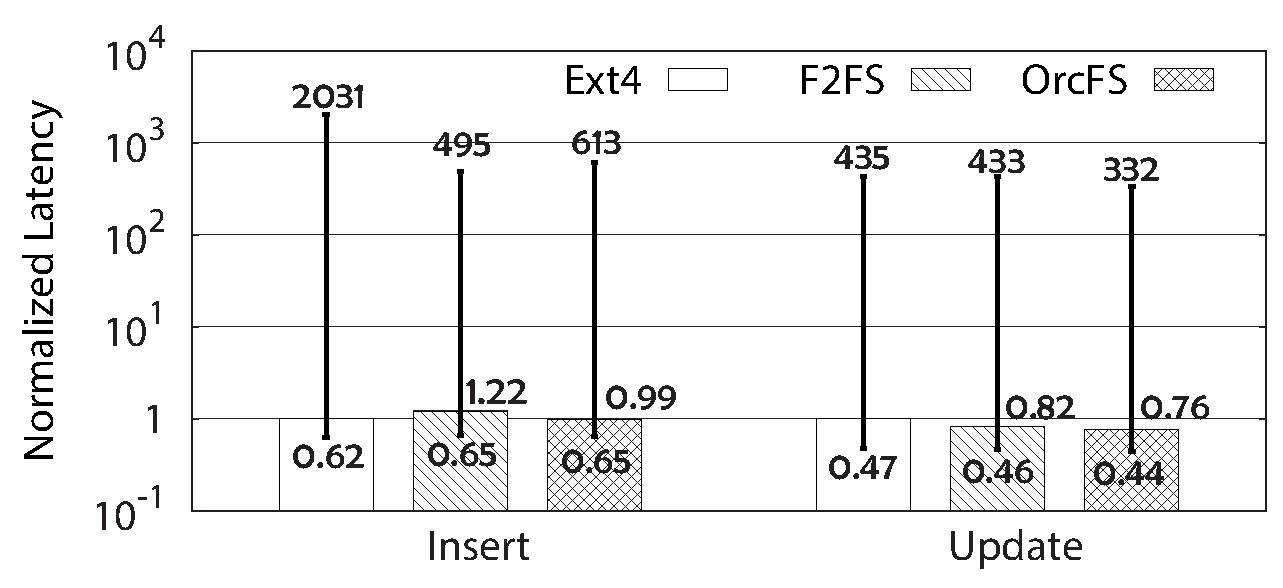
\includegraphics[width=3.2in]{./bench/latency2.eps}
   \label{fig:ycsb_latency}
   }
   \caption{Cassandra (YCSB)\label{fig:ycsb}}
\end{figure}

{\color{red}
Key-Value Store is an important workload in modern data center.
YCSB (Yahoo! Cloud Serving Benchmark)\cite{cooper2010ycsb} provides 
a framework to measure the performance of key-value store. We used 
Cassandra DB \cite{cassandraDB} with YCSB to measure the performance 
of Ext4, F2FS, and OrcFS. Cassandra DB adopts log-structured merge tree \cite{o1996log} 
as its essential data structure. Log-structured merge tree is write-optimized 
search structure and occasional rolling-merge which is equivalent to 
segment cleaning in log-structured filesystem can leave the foreground 
key-value operation under extreme delay. There are two phases in testing 
the performance of Cassandra DB with YCSB. The first phase is `load' that 
inserts records to a empty DB, and the second phase is `run' where YCSB 
generates transactions to measure the performance of the key-value store. 
In load phase, 5,242,880 records with the size of 4 Kbyte is inserted to 
the DB, thus the size of the DB is 20 Gbyte. We used YCSB Workload-A to 
perform read and update operation with ratio of 50:50. 

Fig. \ref{fig:ycsb_throughput} shows the throughput of Insert in load 
phase and overall throughput of read/update operation in run phase. 
The performance of insert in load phase shows 3,554 ops/sec and 3,537 
ops/sec for OrcFS and Ext4, respectively, which is about 20$\%$ higher 
than that of F2FS (2,916 ops/sec). 

When Cassandra is used on top of F2FS, then three layers that is application, 
file system, and SSD firmware keeps a log layer and becomes prone to stacking 
the log problem; thus, the performance of F2FS is lower than the other two 
systems. On the other hand, Ext4 shows about 20$\%$ lower performance than 
OrcFS in run phase. The reason behind the poor performance of Ext4 is due 
to update operation in LSM-tree. To reduce the overhead of searching the 
record in LSM-tree for update operation, it updates a record using `delete 
followed by insert' \cite{o1996log}. As a result Ext4 has to issue \texttt{discard} 
command as much as the number of records updated.

Fig. \ref{fig:ycsb_latency} illustrates the normalized latency of insert 
and update operation in each system. The latency of insert in OrcFS is 
about 18$\%$ lower than that of F2FS, and the latency of update is about 23$\%$ 
lower than that of Ext4. The max latency of insert operation in Ext4 is 568 msec, 
which is about three to four times long than that of F2FS and OrcFS, 
respectivley. Such long latency may cause performance issue in database 
services becuase it has to guarantee the performance consistency as well 
as predictability.
}

\begin{comment}
  \begin{table}[t]
  \begin{center}
    \begin{tabular}{|c|r|r|r|} \hline 
           usec        & Ext4		& F2FS		&	OrcFS	\\ \hline\hline 
  Insert Avg Latency   &  279.8		& 340.4		& 278.6	\\ \hline 
  Insert Min Latency  	&  174 		& 183		& 182	\\ \hline 
  Insert Max Latency 	&  568,319	& 138,495		& 171,391	\\ \hline\hline
  Update Avg Latency   &  259		& 211.9		& 198.2	\\ \hline
  Update Min Latency  	&  122 		& 120		& 114	\\ \hline 
  Update Max Latency 	&  112,703	& 112,319		& 86,015	\\ \hline

  \end{tabular}
  \end{center}
  \vspace{-0.7em}
  \caption{YCSB Insert, Update Latency (usec, 20 GByte Cassandra DB, 4 KByte Record Size)}
  \label{tab:ycsb}
  \end{table}
\end{comment}


\begin{comment}
  \begin{figure}[t]
  \centering
   \subfloat[w/o QPSC (Runtime: 860 sec)]{
   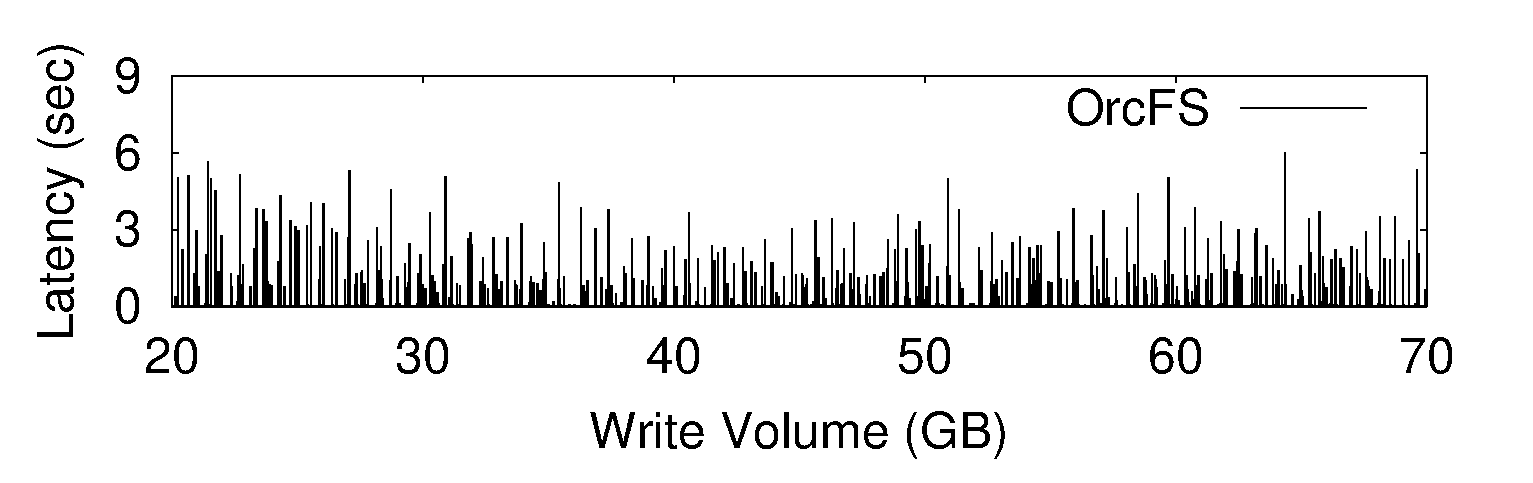
\includegraphics[width=1.6in]{./qpsc/normal_latency.eps}
   \label{fig:lat_wo_qpsc}
   }
   \subfloat[w/ QPSC (Runtime: 480 sec)]{
   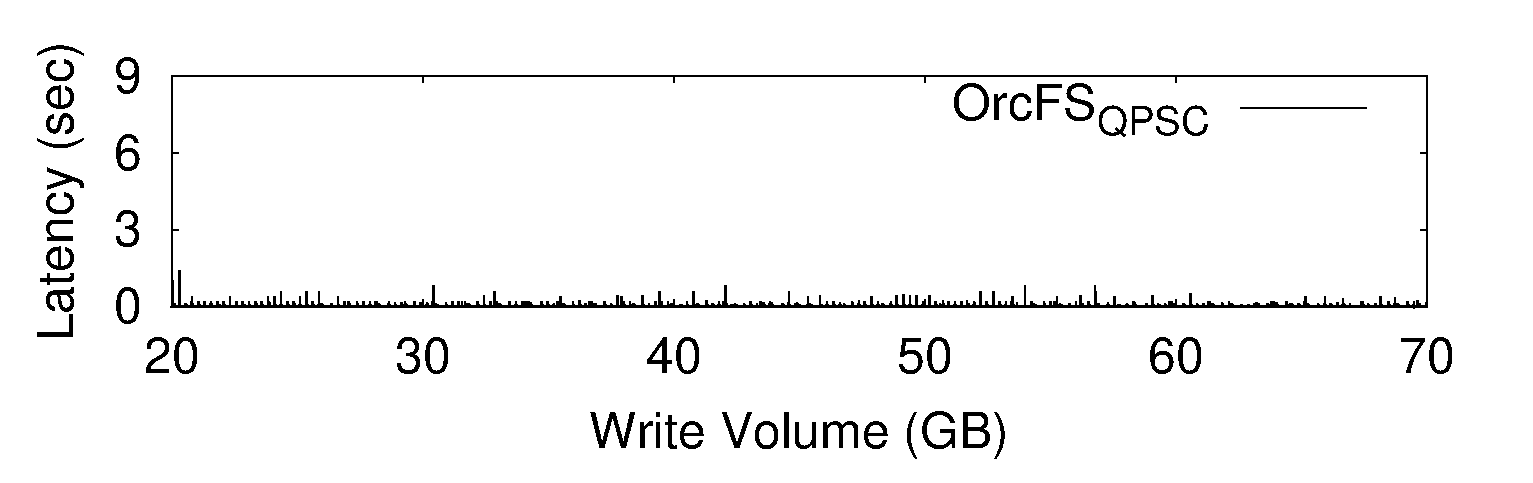
\includegraphics[width=1.6in]{./qpsc/qpsc_latency.eps}
   \label{fig:lat_w_qpsc}
   }\quad
   \subfloat[CDF of Segment Cleaning Latency]{
   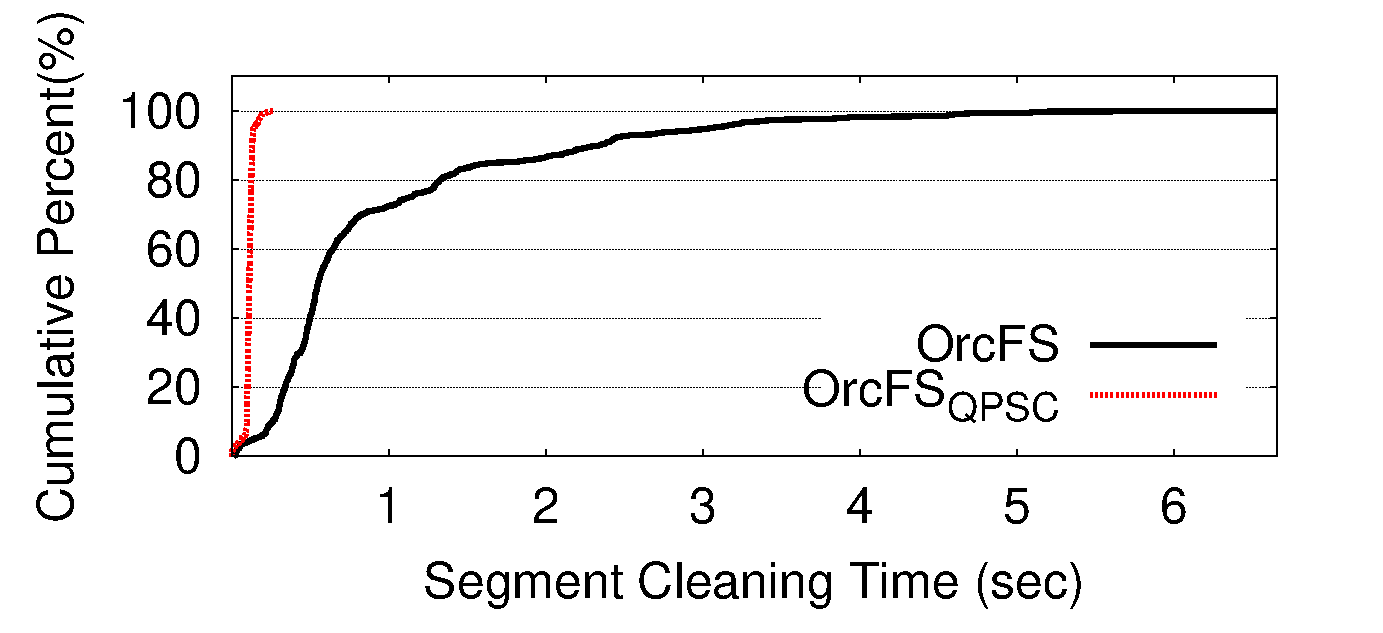
\includegraphics[width=3.2in]{./qpsc/usl_qpsc_cdf.eps}
   \label{fig:lat_qpsc_cdf}
   }
   \caption{Write Latency (110 Gbyte Cold File, 80 Gbyte Hot File, 4 KByte Buffered Random Write to Hot File)\label{fig:lat_qpsc}}
  \end{figure}
\end{comment}

\begin{figure}[t]
  \centering
   \subfloat[w/o QPSC (Runtime: 860 sec)]{
   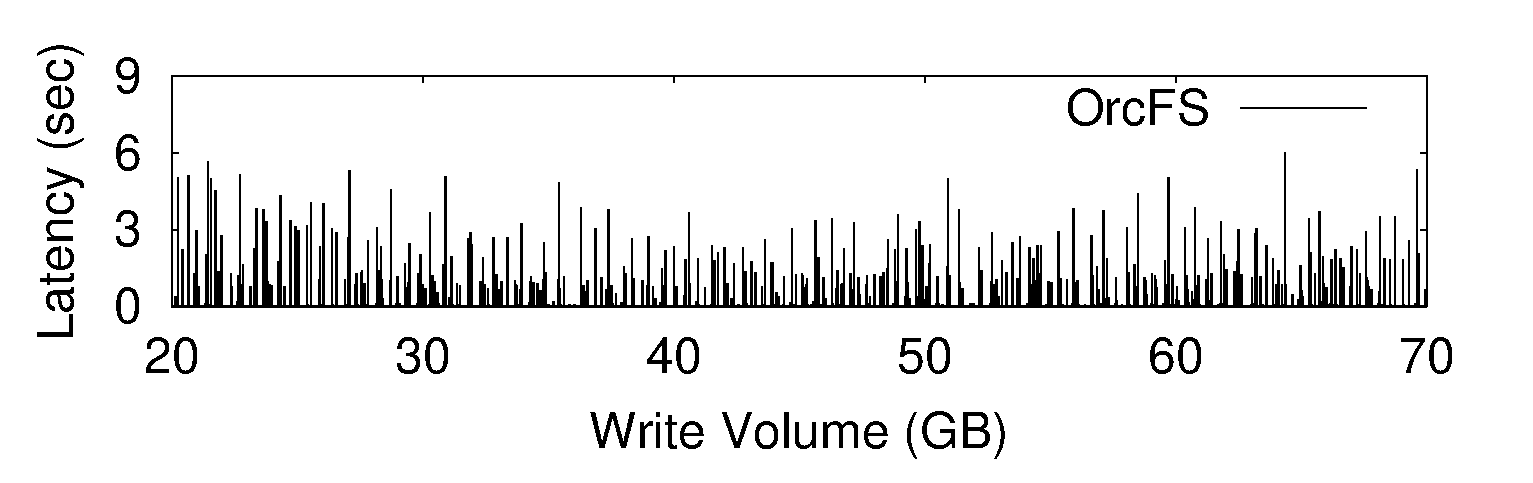
\includegraphics[width=3.5in]{./qpsc/normal_latency.eps}
   \label{fig:lat_wo_qpsc}
   }\quad 
   \subfloat[w/ QPSC (Runtime: 480 sec)]{
   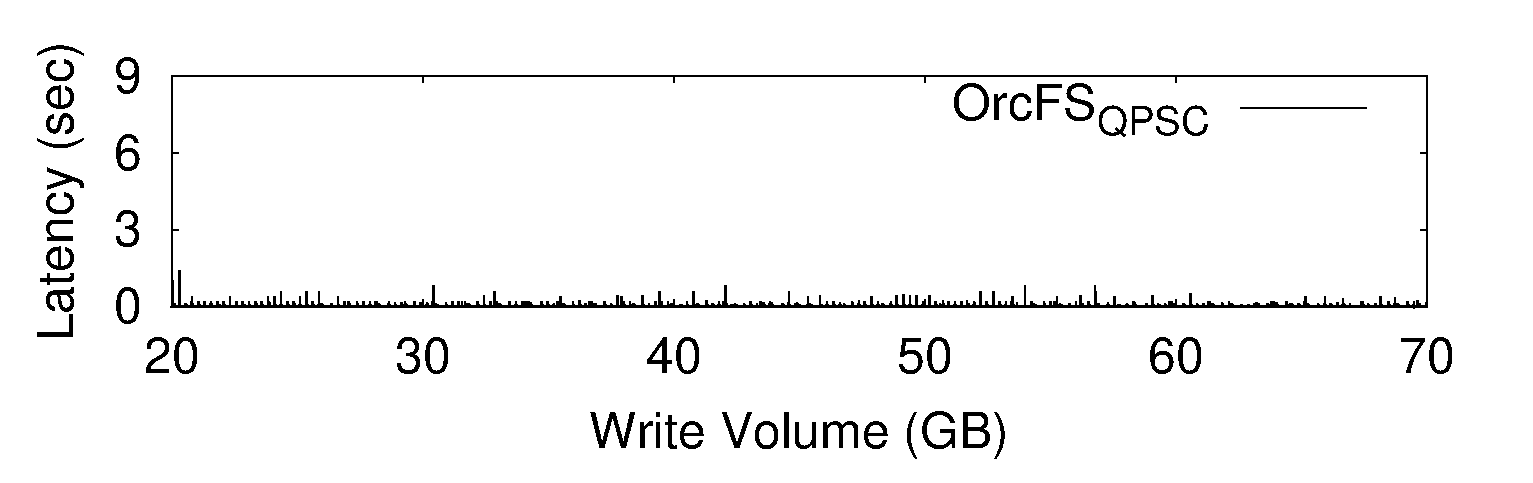
\includegraphics[width=3.5in]{./qpsc/qpsc_latency.eps}
   \label{fig:lat_w_qpsc}
   }
   \caption{Write Latency (110 Gbyte Cold File, 80 Gbyte Hot File, 4 KByte Buffered Random Write to Hot File)\label{fig:lat_qpsc}}
\end{figure}

\begin{table}[t]
  \begin{center}
  \begin{tabular}{|c|c|c|c|c|c|} \hline
   				& Avg 		& 99\%	& 99.9\% 		& 99.99\% 	& Max 	\\ \hline\hline
  OrcFS			& 44 us		& 11	us	& 36 us		& 21 ms		& 8.9 sec	\\ \hline
  OrcFS$_{QPSC}$	& 43 us		& 10	us 	& 11 ms		& 70 ms 		& 1.4 sec	\\ \hline
  \end{tabular}
  \end{center}
  \caption{Quartile Information of Write Latency (us: microsecond, ms: millisecond)}
  \label{tab:qpsc_latency}
\end{table}


\subsection{Quasi-Preemptive Segment Cleaning}
\label{subsec:qpsc_test}

We examine the effect of segment cleaning over foreground IO. We perform 
buffered write() and create a situation where there runs out of free section. 
The section size is 256 Mbyte. When there runs out of free section, the segment 
cleaning module of both F2FS and OrcFS cleans the sections until it creates at 
least one additional section. If the section utilization is $\rho$, it needs 
to clean $\frac{1}{1-\rho}$ sections to create one additional free sections. 
If  $\rho$ is 0.6, the segment cleaning module consolidates the blocks from 
at least three sections. With 256 Mbyte section, it has to scan 800 Mbyte of 
filesystem blocks and migrates nearly 600 Mbyte of data blocks to a destination 
section. If this operation interferes with the ongoing IO, the application may 
experience intolerable amount of delay. We examine the latency of 4 Kbyte 
buffered write() operation. 

We set the polling interval to 100 m sec. Fig. \ref{fig:lat_qpsc} illustrates the result. 
We only shows the interval where the segment cleaning is active. As can be 
seen, without proper management, the latency of 4 Kbyte write() can be as 
high as 9 sec. It is prohibitive. With 100 m sec polling interval in Quasi 
Preemptive Segment Cleaning, we cannot observe any abnormal delay which has 
been observed in F2FS. Table \ref{tab:qpsc_latency} illustrates the tail statistics of the 
write latency. F2FS yields unto 8.9 sec IO latency. In OrcFS, the latency 
of write operation is less than one sec. Further, 99.99\% point value 
corresponds to 21 msec and 38 msec in F2FS and OrcFS, respectively. Quasi-Preemptive 
Segment Cleaning successfully resolves the excessive segment cleaning 
overhead which may appear in large size section based space management.
{\color{red} qpsc가 실행시간이 짧은 이유 분석바람.}

\begin{comment}
{\color{red}
We examine the effectiveness of the QPSC by measuring the latency of
\texttt{write()} system call in the following workload where segment
cleaning is triggered frequently.  In the experiment, the cold data is
110 Gbyte and the hot data is 80 Gbyte.  After creating the cold and
hot data, we overwrite 70 Gbyte of the hot data with buffered 4 Kbyte
random write.  Fig. \ref{fig:lat_qpsc} shows the write latency due to
segment cleaning.


The result is clear. Using NPSC on a system with a large section size
as the unit of segment cleaning is very ineffective.  The average
write latency is 44 usec and the maximum time shows as long as 8.9
sec. On the contrary, the average and the maximum write latency on
QPSC is 25 usec and 1 sec, respectively.  The write latency is
shorter in QPSC because it has the ability to handle outstanding host
user I/O requests.  Another unseened effect of using QPSC is the total
run time.  The total run time of QPSC is only 480 sec whereas the NPSC
shows 860 sec.  The overall run time is reduced because the QPSC
allows lowering the victim section utilization.
}
\end{comment}

\begin{comment}
We examine the effectiveness of the Quasi-Preemptive Segment Cleaning.

We observe that OrcFS with Quasi-Preemptive Segment Cleaning (QPSC) reduces the response time of host I/O requests. To test the effect of QPSC on response time use created a cold and a hot file with the size of 110 Gbyte and 80 Gbyte, respectively. We measured the 4Kbyte buffered random write to overwrite 70 Gbyte of the hot file while measuring the latency of segment cleaning. Fig. \ref{fig:lat_wo_qpsc} shows the latency of OrcFS without the preemption in segment cleaning, and Fig. \ref{fig:lat_wo_qpsc} shows the latency of QPSC enabled OrcFS (OrcFS$_{QPSC}$). Fig. \ref{fig:lat_qpsc_cdf} shows the CDF of segement cleaning latency in OrcFS and OrcFS$_{QPSC}$.

Maximum segment cleaning latency shown in Fig. \ref{fig:lat_wo_qpsc} is 6.6 sec, which infers that the response time for a write request from the host can be as long as 6.6 sec. On the contrary, Fig. \ref{fig:lat_w_qpsc} shows that latency of OrcFS$_{QPSC}$ exhibits as long as 278 msec and handles host I/O requests with higher priorities. The average write latency of OrcFS is 929 msec and OrcFS$_{QPSC}$ is 111 msec that is reduction of 88$\%$. As can be observed from comparing Fig. \ref{fig:lat_wo_qpsc} and Fig. \ref{fig:lat_w_qpsc}, OrcFS$_{QPSC}$ shows lower variance in segment cleaning latency proving that OrcFS$_{QPSC}$ provides better predictability. 

An other interesting point that can be observed in the result is that OrcFS$_{QPSC}$ shows 44$\%$ shorter execution time than OrcFS, that is reduction from 860 sec to 480 sec. It is because OrcFS$_{QPSC}$ processes host I/Os first, which increases the number of invalid blocks. When the time comes to select a victim section, it has higher chance of choosing a section with low utilziation which increases the efficiency of segment cleaning. The result clearly shows that QPSC not only significantly reduces the system blocking time incurred by segment cleaning but also increases the efficiency of segment cleaning. 

\end{comment}

\begin{comment}
  \begin{table}[t]
  \begin{center}
  \begin{tabular}{|r|r|r|r|r|r|} \hline
  	     	& Min	& Avg 		& 99.9\% 		& Max 		\\ \hline\hline
  OrcFS	(msec)    		& 15.6 & 929.2 & 5,734.6 & 6,651.9 	\\ \hline
  OrcFS$_{QPSC}$ (msec)	& 1.2 & 111.3	& 252.6 & 278.4	\\ \hline
  \end{tabular}
  \end{center}
  \vspace{-0.7em}
  \caption{OrcFS Segment Cleaning Latency according to Quasi-Preemptive Segment Cleaning (msec)}
  \label{tab:lat_qpsc}
  \end{table}
\end{comment}

\subsection{Effect of Eliminating the Redundancies}
\label{subsec:remove_gc_overhead}

OrcFS eliminates the redundancies in the address translation across 
the layers. Different regions of the storage are managed by different 
layers of the storage stack: data region by the host filesystem and the 
metadata region by the storage device, respectively. The benefit is 
clear. There will be no compound storage consolidating effort. We measure 
the effectiveness of eliminating the redundancies from the perspective of 
write amplification as well as from the perspective of the performance. 
The workload are carefully crafted to trigger the garbage collection at 
the storage device as well as at the segment cleaning at the filesystem. 
The hot region size is sufficiently large so that ???{\color{red} 각 
region의 크기에 따른 waf의 영향 간단히 설명}

The garbage collection and the segment cleaning behavior is governed by 
the free space at the filesystem, the size of the overprovisioined area 
at the Flash storage, For 256 GByte SSD, we create 170 Gbyte file. For 
170 GByte file, we designate the half of the file as hot region. We  
perform random write only to the host region of the file. A single iteration 
ends if all blocks are over-written. Random writes (buffered 4 Kbyte write) 
are created so that each of the file blocks in the host region is written 
one and only once. We run the fifteen iterations of this workload. Write 
amplification is measured using smartmontools \cite{smartmontools}.

First, we examine the performance. F2FS and OrcFS yield 53K IOPS and 75K IOPS, 
respectively (Fig. \ref{fig:f2fs_vs_usl_iops}). OrcFS shows 45\% performance gain against F2FS. Second, we 
examine the write amplification created by each layer. Fig. \ref{fig:f2fs_vs_usl_waf} illustrates 
the result. In the filesystem level, F2FS and OrcFS amplifies the write by 
1.13 and 1.3, respectively. Due to the larger segment cleaning unit size, it 
is inevitable that OrcFS inefficiently consolidates the file blocks and 
therefore has larger write amplification. SSD in F2FS and SSD in OrcFS exhibit 
stark contrast. In F2FS, the underlying SSD amplifies the write operation 
by 1.56. This is due to garbage collection at the storage device. On the other 
hand, in OrcFS, since the filesystem is in charge of consolidating the physical 
NAND flash storages, the storage device itself does not entail any amplification. 
The segment cleaning at the filesystem and the garbage collection at the storage 
device compounds. F2FS and OrcFS yields 1.76 and 1.3 write amplification seen 
from the storage device. OrcFS eliminates 1/4 of the write volume.

Third, we analyze the cause for this amplification. Fig. \ref{fig:io_distribution} illustrates the 
result. The application creates 85 GByte of write to the filesystem data 
region in both F2FS and OrcFS. In F2FS and OrcFS, the filesystem creates 431 Mbyte 
and 599 Mbyte of metadata update, respectively. {\color{red} why OrcFS creates more 
metadata update?}. In F2FS, we observe that Flash storage creates huge amount 
of writes by itself due to garbage collection. Meanwhile, OrcFS is free from 
this behavior yielding much more efficient storage behavior.

The write volume governs the lifespan of the Flash storage. Roughly, 
eliminating the 1/4 of total write volume lead to the 30\% extension of the lifespan.

\begin{figure}[t]
  \centering
  \subfloat[WAF]{
    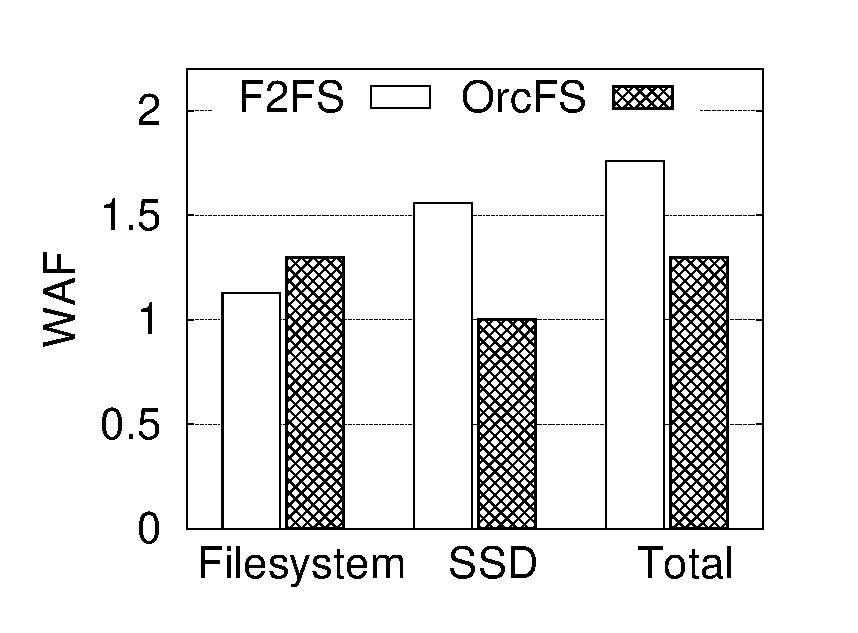
\includegraphics[width=2in]{./comp_gc/f2fs_vs_usl_waf}
   \label{fig:f2fs_vs_usl_waf}
   }
   \subfloat[IOPS]{
   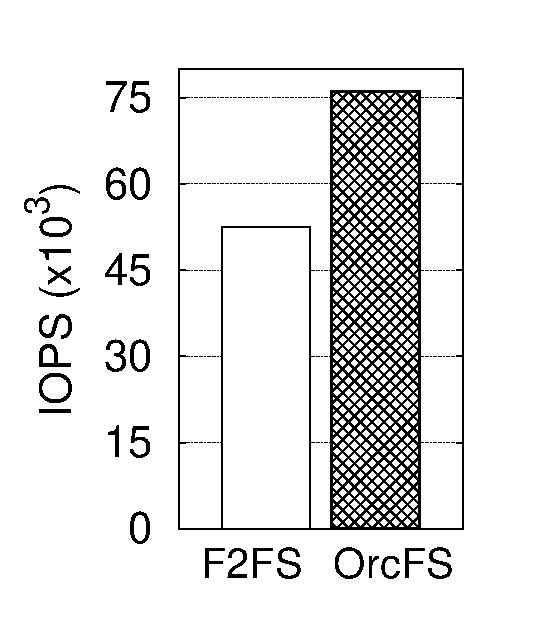
\includegraphics[width=1in]{./comp_gc/f2fs_vs_usl_iops}
   \label{fig:f2fs_vs_usl_iops}
   }
   \caption{WAF and IOPS of Each System
     (85 Gbyte Cold File, 85 Gbyte Hot File, 4 Kbyte buffered random write to the Hot File, 170 Gbyte Total write volume, Section size of F2FS: 256 Mbyte)\label{fig:f2fs_vs_usl}}

\end{figure}

\begin{comment}
\begin{figure*}[t]
\label{fig:170_85_randw}
\centering

\subfloat[File System WAF]{
 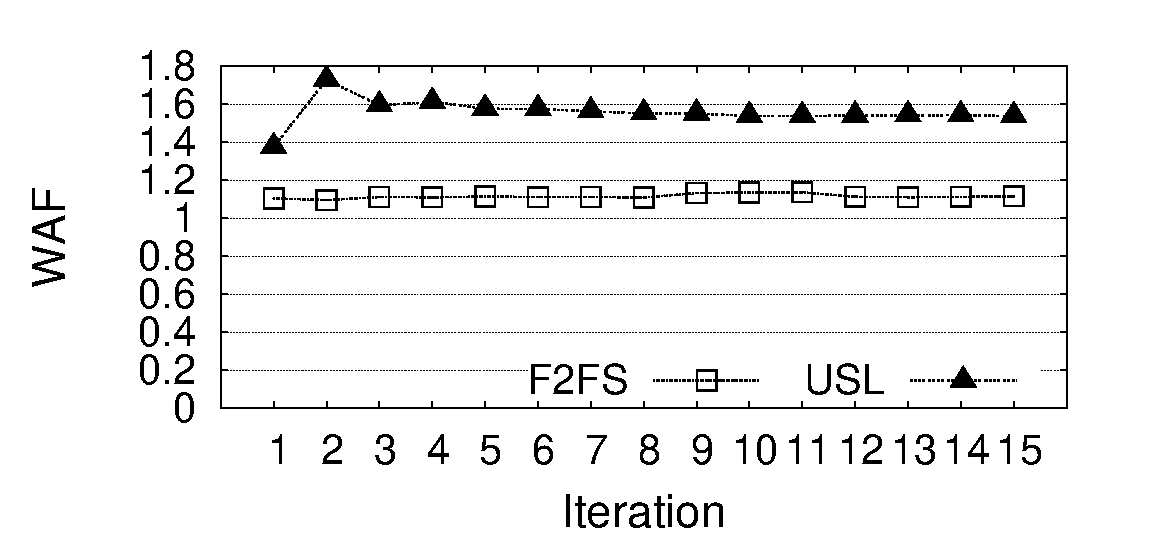
\includegraphics[width=3.3in]{./comp_gc/170_85_randw_fs}
 \label{fig:170_85_randw_fs}
 }
\subfloat[Device WAF]{
 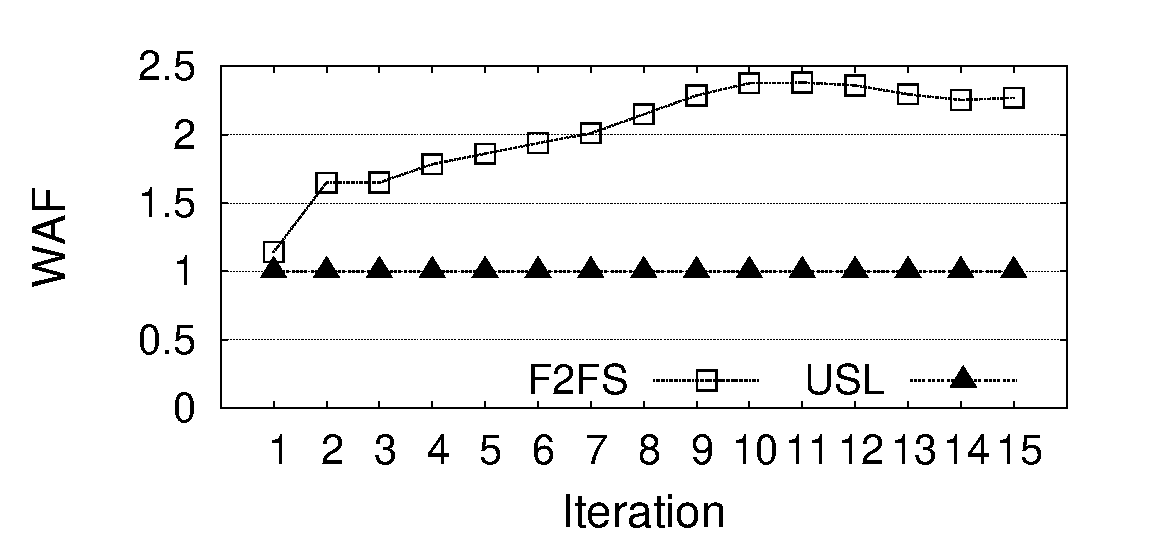
\includegraphics[width=3.3in]{./comp_gc/170_85_randw_dev}
 \label{fig:170_85_randw_dev}
 }
\subfloat[Total WAF]{
 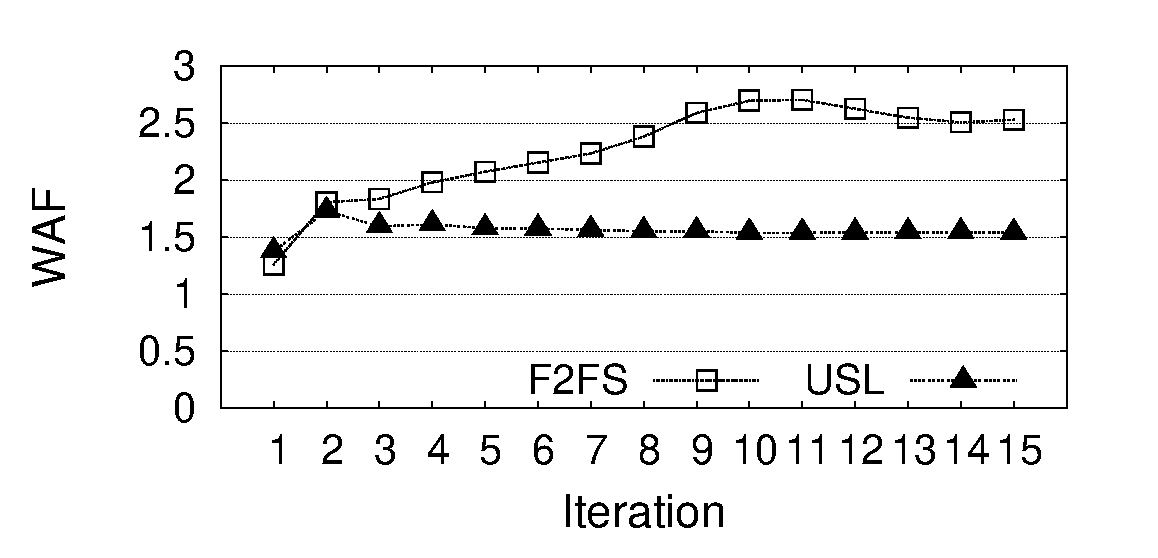
\includegraphics[width=3.3in]{./comp_gc/170_85_randw_total}
 \label{fig:170_85_randw_total
 }
 \subfloat[IOPS]{
 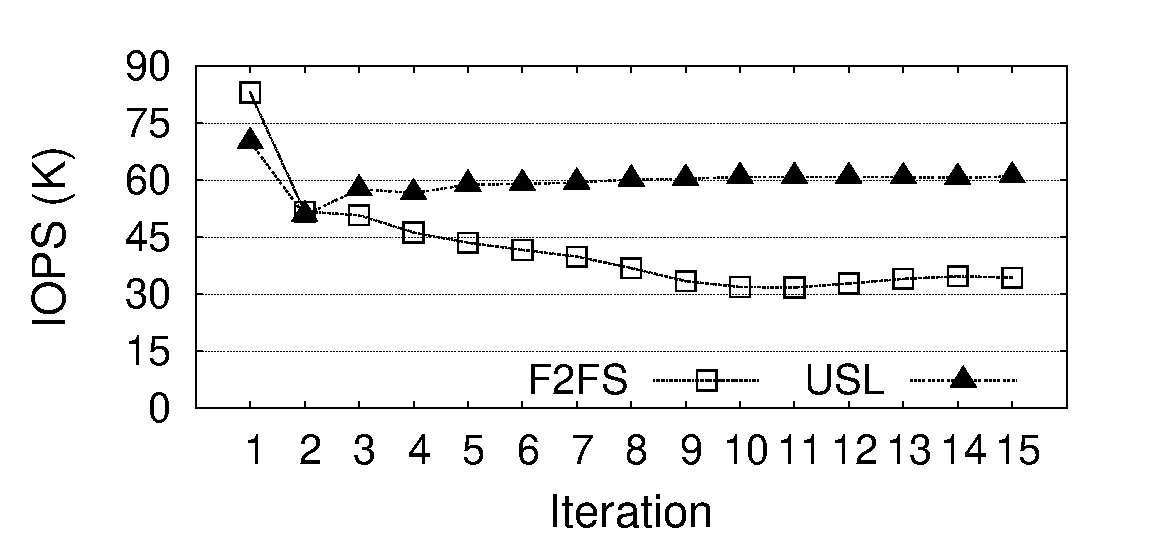
\includegraphics[width=3.3in]{./comp_gc/170_85_randw_iops}
 \label{fig:170_85_randw_iops}
 }
 \caption{The Result of Compound Garbage Collection in Case Study 2
   (Section size of F2FS: 256 Mbyte)\label{fig:170_85_randw}}
\end{figure*}
\end{comment}




\begin{figure}[t]
\begin{center}
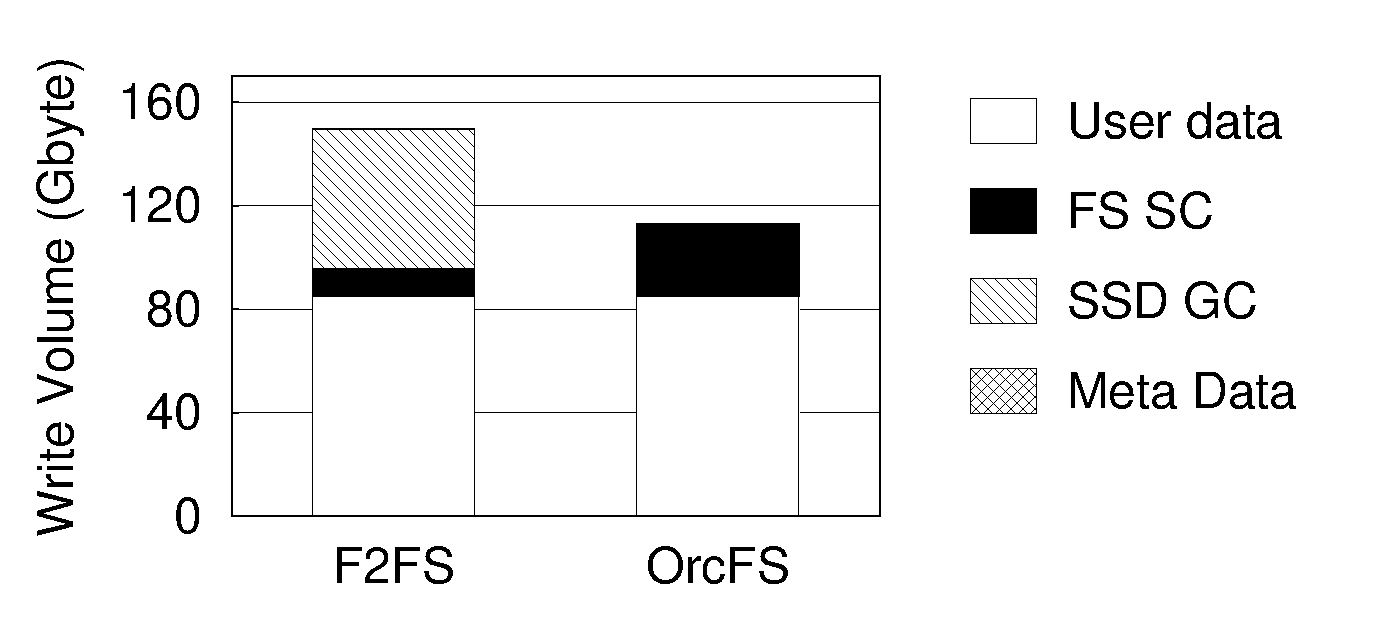
\includegraphics[width=3.2in]{./comp_gc/io_distribution.eps}
\caption{Total Write Volume Distribution (4 Kbyte buffered random write, Write volume generated by the application is 85 Gbyte, Section size of F2FS: 256 Mbyte)}
\label{fig:io_distribution}
\vspace{-1.5em}
\end{center}
\end{figure}


\begin{comment}
  \begin{figure}[t]
  \begin{center}
  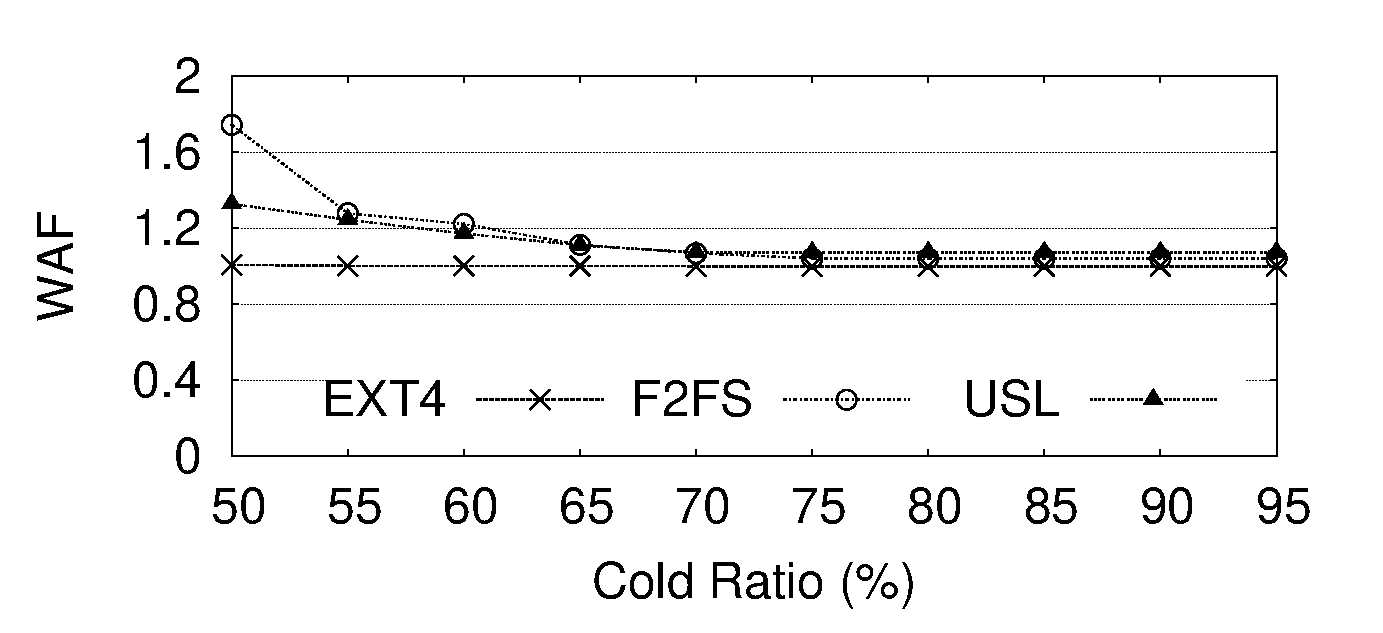
\includegraphics[width=3.2in]{./comp_gc/cold_ratio_waf.eps}
  \caption{WAF according to the Cold Data Ratio (The total size of cold data and hot data is 170 Gbyte, Section size of F2FS:    256 Mbyte)}
  \label{fig:cold_ratio_waf}
  \vspace{-1.5em}
  \end{center}
  \end{figure}
\end{comment}

\subsection{RW: Cold block ratio and Segment Cleaning Overhead}
\label{section:cbr}

{\color{red}

In this section, we examine the file system performance with respect
to the hot and cold data ratio in the system. The volume of the hot
data ($F_{hot}$) used in the experiment is dependent on the the volume
of the cold data ($F_{cold}$). $F_{hot}$ is set using the following
equation: $TotalVolume \times ( 1 - x ) = F_{hot}$, where
$TotalVolume$ is the sum of hot and cold data created on the
partition, and $x$ is the ratio of cold data in $TotalVolume$. We set
$TotalVolume$ as 170 and vary the $x$ from 0.5 to 0.95. We use
buffered 4 Kbyte random write on $F_{hot}$ as one iteration, and we
use the average performace of 15 iterations. The result is shown in
Fig. \ref{fig:cold_ratio_iops}.

When $F_{hot}$ is set to 50$\%$ of the $TotalVolume$, the performance
of F2FS and OrcFS is lower than the performance of EXT4.  It is
because the overhead of segment cleaning in log-structured systems
increases as the size of the hot data increases.  On the other hand,
the performance of EXT4 does not vary with respect to the cold ratio
in the system, because it writes in in-place update manner.  When the
cold ratio is set to 55$\%$, OrcFS crosses the performace of EXT4, and
from then on OrcFS outperforms EXT4 and F2FS on all the
cases. The performance of OrcFS at cold ratio of 95$\%$ shows 45$\%$
better performance than that of EXT4.  Considering the report that the
size of the hot data in the system is about 5 to 25$\%$ of the
workload \cite{park2011hot}, it is reasonable to say that the
performance of OrcFS is superior to other systems.  
}


\begin{comment}

In most storage devices, the dominant fraction of the storage is filled
with cold files which are barely updated or accessed \cite{park2011hot}. We
examine the performance of different storage stacks varying the fraction
of cold data over entire storage partition.

Fig. \ref{fig:cold_ratio_iops} shows the result of 4 Kbyte buffered
random writes to the hot file on three file systems while varying the size of cold data. 
The relationship between hot file size ($F_{hot}$), cold file size ($F_{cold}$), 
and the total volume ($TotalVolume$) in Gbytes used in the experiment is as follows: 
$F_{cold} + F_{hot} = TotalVolume$ and $TotalVolume \times ( 1 - x ) = F_{hot}$.
We set $TotalVolume = 170$ and $x$ equals to ratio of $TotalVolume$, 
which we vary from 50$\%$ to 95$\%$. For example, when $TotalVolume = 170$ 
and $x = 0.6$, the size of hot data is $170 \times 0.4 = 68$ Gbyte and 
the cold data is 102 Gbyte. We repeat the experiment fifteen times, and the total
volume written in an iteration is 170 Gbyte. The result shows the average of fifteen iterations. 

In all cases, OrcFS outperforms the result of F2FS; OrcFS is about 21$\%$
faster than F2FS when the cold ratio is 50$\%$ and the difference
closes into 4$\%$ when the cold ratio becomes 95$\%$. It shows that the
effect of compound garbage collection becomes less significant as the
hot ratio becomes smaller. The performance of Ext4 is stable around 83.5 $\sim$ 86.5
KIOPS. The performance of OrcFS becomes higher than Ext4 when the cold
ratio is less than 55$\%$ and the gap widens as the ratio
decreases. When the cold ratio set to 95$\%$, OrcFS shows about 41$\%$
higher IOPS than that of Ext4. Considering the report that the size
of the hot data in the system is about 5 to 25$\%$ of the workload
\cite{park2011hot}, it is reasonable to say that the
performance of OrcFS is superior to other systems, especially when most
of the partition is filled with cold data and only small amount of
data is frequently accessed. 

\end{comment}

\begin{figure}[t]
\begin{center}
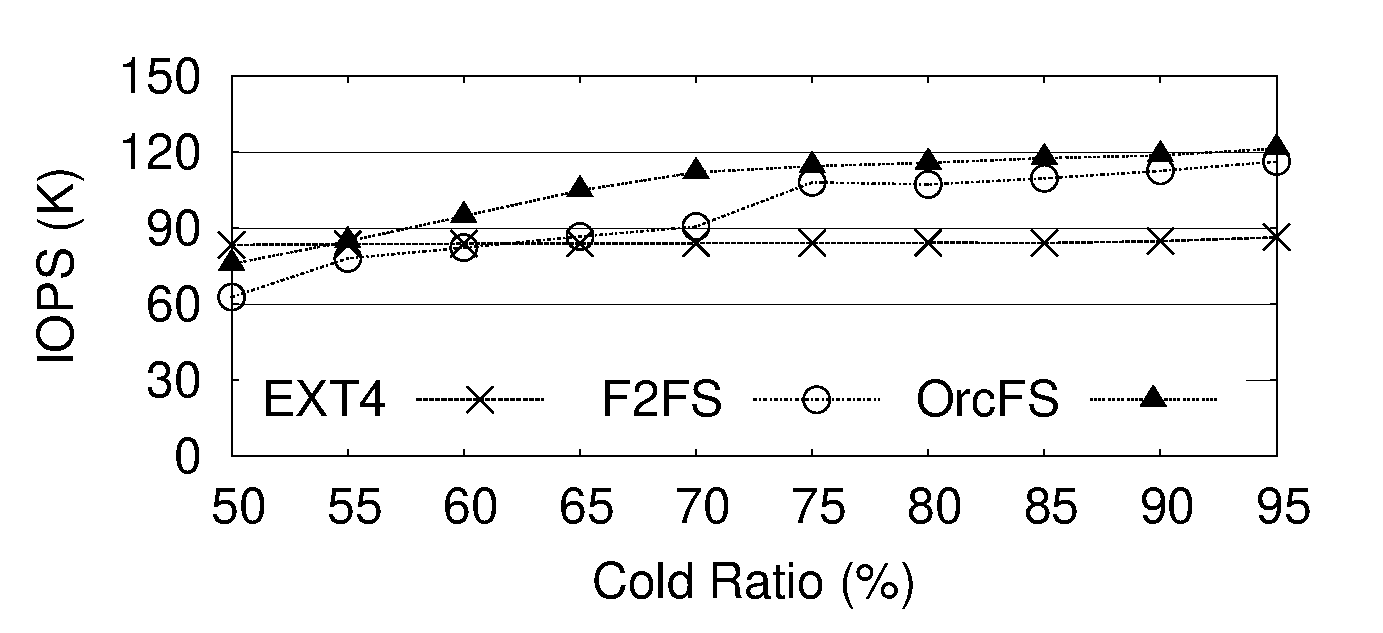
\includegraphics[width=3.2in]{./comp_gc/cold_ratio_iops.eps}
\caption{Random Write Performance according to the Cold Data Ratio (The total size of cold data and hot data is 170 Gbyte, Section size of F2FS: 256 Mbyte)}
\label{fig:cold_ratio_iops}
\end{center}
\end{figure}

\begin{comment}
  Fig. \ref{fig:cold_ratio_waf} shows the WAF of systems observed in
  measuring the performance for Fig. \ref{fig:cold_ratio_iops}. The WAF of a
  system is measured by multiplying the WAF of file system to the WAF of
  the storage. Overall, the result shows that 
  the system WAF with F2FS is higher than the system WAF with OrcFS. As it is described in
  \cref{subsec:remove_gc_overhead}, F2FS has higher WAF than other systems
  because of the write amplification caused by compound garbage collection.
  It has to be noted that although the system WAF with Ext4 is the lowest, but IOPS on
  OrcFS is higher than that of Ext4. It is because all random writes in OrcFS are
  sequentially logged to the storage.

  The proposed OrcFS with disaggregate mapping allows not only reducing the
  device level garbage collection but also lowering the total WAF of the
  system.
\end{comment}


\subsection{Block Patching Overhead}
\label{subsec:patching_overhead_test}

Block patching module aligns the IO size with the Flash page size via 
padding empty page cache entries. It consumes one page cache entry. Depending 
on the nature of the workload, the space overhead of the block patching can 
vary widely. We examine the block patching overhead in three workloads which 
we have used in this study: random write, varmail and YCSB workload. Each of 
these workloads has widely different access characteristics. YCSB benchmark 
uses log-structured merge tree which flushes the dirty page cache entries in 
the unit of tens of Mbyte. Therefore, the overhead of block patching is negligible (0.3\%). 
On the other hand, vermeil workload frequently calls \texttt{fsync()} to synchronize the 
updated file metadata to the storage. In this workload, block patching entails 
28\% overhead. For random write, the block patching overhead is 2\%.

\begin{table}[t]
  \begin{center}
  \begin{tabular}{|c|c|c|>{\columncolor[gray]{0.9}}c|} \hline
  Workload 							& Dummy Write	& Total Write	& Ratio 		\\ \hline\hline
  varmail	 (\cref{subsec:micro_bench})	& 514 MB		& 1.8 GB		& 28\%	\\ \hline
  YCSB (\cref{subsec:ycsb_bench})		& 196 MB		& 74 GB		& 0.3\%	\\ \hline
  Rand W (\cref{subsec:remove_gc_overhead}) & 2 GB		& 113 GB		& 2\%	\\ \hline
  \end{tabular}
  \end{center}
  \caption{Block Patching Overhead}
  \label{tab:block_patching}
\end{table}



\begin{comment}
  \begin{figure}[t]
  \begin{center}
  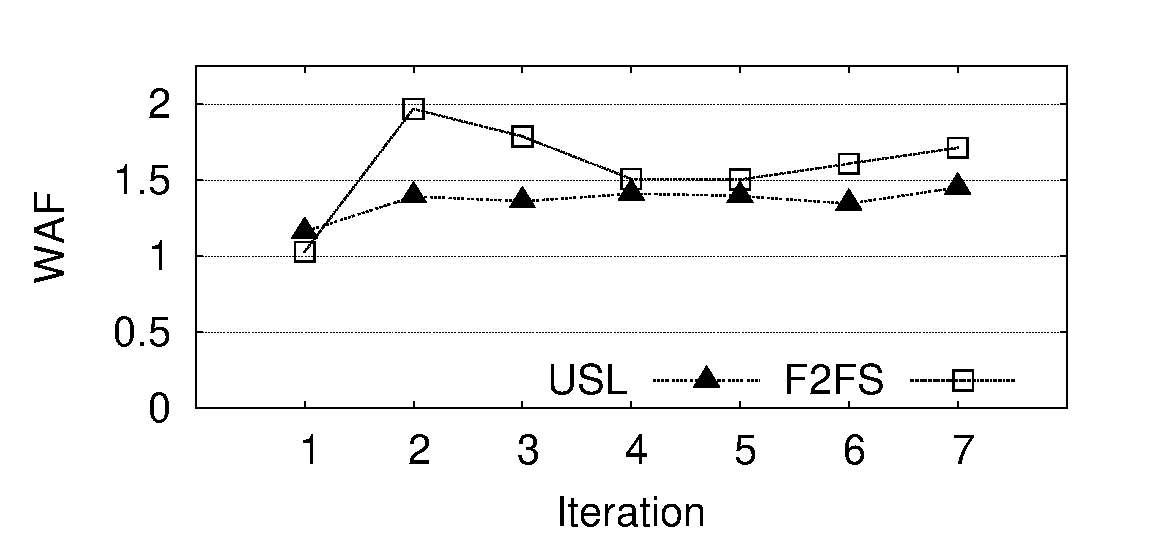
\includegraphics[width=3.5in]{./comp_gc/50_50_seqw_total}
  \caption{The Result of Compound Garbage Collection Scenario 3 (Section
    size of F2FS: 256 Mbyte)}
  \label{fig:50_50_seqw_waf}
  \vspace{-1.5em}
  \end{center}
  \end{figure}
\end{comment}


\section{Related Works}
\label{sec:related_works}

\paragraph{Flash based File System: }
There are number of efforts, such as YAFFS \cite{manning2010yaffs},
JFFS2 \cite{zhang2006implementation}, LogFS \cite{engel2005logfs}, and
UbiFS \cite{hunter2008brief}, to manage the raw Flash device in the
host side.  Since it does not have a Flash Translation Layer (FTL) in
the device, the host file system has to provide the mechanism for bad
block management, wear-leveling, and garbage collection. Moreover,
they only support one Flash memory device. 

FusionIO introduced Direct File System, DFS \cite{josephson2010dfs}
which is a file system for a high-performing SSD.  DFS keeps
Virtualized Flash Storage Layer to manage block allocation and inode
management that used to be the role of the file system. And, becuase
DFS directly manages the mapping of the SSD, it does not suffer from
compound garbage collection problem.

\paragraph{Reducing the Metadata Overhead: }

Both the file system and the storage device has to keep mapping
information. In order to relieve the burden of the device memory
requirement, FSDV (File System De-Virtualizer) \cite{zhangremoving}
provides a way for the host to manage the physical address mapping
information. It achieves to reduce the mapping table management
overhead by removing the logical to physical address mapping
information on SSD. 

Unlike FSDV which removed the overhead of device mapping information,
NVMKV \cite{nvmkv} removes the host side metadata management overhead
by replacing FTL commands with key-value operations. NVMKV uses
commands like atomic multiple-block write, p-trim, exits, and iterate,
as the interface to the Flash device. 


\paragraph{Host Managed Storage System: }
ANViL \cite{anvil} lets the host modify logical-to-physical mapping
information on device through new I/O interfaces. The host exploits
the given interfaces to remove the redundant data copy overhead. It
also provides useful features such as single journaling and file
snapshot to the system.

\paragraph{Compound Garbage Collection: }
The compound garbage collection problem on stacked log system is first
enlighted by Yang et al. \cite{yang2014don}. Since then Baidu
introduced SDF (Software-defined Flash) \cite{sdf}, Lee et
al. introduced AMF (Application Managed-Flash)
\cite{lee2016application}, and Zhang et al. proposed
ParaFS\cite{zhang2016parafs}.


AMF (Application Managed-Flash) \cite{lee2016application}, which is
based on F2FS \cite{lee2015f2fs}, exploits the fact that
log-structured applications always append the data to reduce the size
of metadata for Flash based sotrages. AMF modified the metadata area
of F2FS so that it is also managed in log-structured manner; thus, can
exploit the block mapping in the storage layer. Since both layers of
the file system and the Flash device can use block mapping, it gives a
partial solution to the compond garbage collection problem.

ParaFS\cite{zhang2016parafs} acquires hardware information for the
storage to identify the number of channels the device has. ParaFS
exploits the information to distribute the data according to their
hotness and maximize the channel parallelism.  It also implements
coordinated garbage collection scheme and parallelism aware scheduling
to solve the compound garbage collection and load balancing.


\section{Conclusion}
\label{sec:conclusion}

Modern IO stack is full of unnecessary redundancies with duplicate efforts 
across the layers: the storage device, host filesystem and even the application. 
To fully exploit the append-only and asymmetric read/write  nature of the Flash 
storage device, these three layers endeavor to align their behavior to the physical 
characteristics of the Flash storage. Each of these layers introduces the level 
of indirection maintaining its own address translation information using 
log-structured filesystem or using append-only search structure such as 
log-structured merge tree. Subsequently, each of the filesystem and the storage 
device reserves a certain fraction of its space to consolidate the invalid blocks. 
This duplicate efforts leads to the waste of the storage space, increase in the 
write-amplification and performance degradation. In this work, we propose OrcFS, 
Orchestrated Filesystem which orchestrates the behavior of the Flash friendly 
filesystem and the flash storage. OrcFS partitions the storage space into two 
regions and assigns the management role of individual partitions to different 
layers of the stack: filesystem and the storage device. OrcFS fully exploit the 
internal parallelism of the underlying flash storage ( multi-channel and multi-way) 
via making the unit of segment cleaning equivalent to the superblock of the 
underlying Flash storage. Novel Quasi-preemptive segment cleaning algorithm 
effectively resolves the excessive IO delay which may entail due to large segment 
cleaning unit size. The engineering implication of the OrcFS is impressive. 
It reduce the device mapping table size to 1/56 and to 1/4 from the page mapping 
and from the smallest mapping table size proposed in the literature, ParaFS. 
Despite its minimal hardware resource requirement, the OrcFS exhibits superior 
performance against EXT4 and F2FS over page mapping based SSD in broad range 
of workloads; in synchronous random write dominant workload, \texttt{varmail} 
as well as, append-only asynchronous write dominant workload such as YCSB. 
Via eliminating the compound segment cleaning efforts in the filesystem and in 
the storage device, we eliminate 1/4 of the write volume to the storage device 
leading to the 30\% extension of its lifespan.

%\bibliographystyle{IEEEtran}
%\bibliographystyle{acm}
%\bibliographystyle{unsrt}
\bibliographystyle{plain}
\bibliography{ref}

%\pagebreak
%\tableofcontents

\section{Appendix}

While append-only nature of the Flash memory fits well with 
the log-structured file system, they have drawbacks. When 4 KByte followed 
by \texttt{fsync()} is called in NILFS, it flushes a segment with 128 KByte \cite{Jeong2013stack}. 
Most of the log-structured file system blindly places the file data and the 
associated metadata in proximity as an effort to reduce the seek-time overhead. 
However, file data and file metadata have entirely different update frequency. 
For Flash storage, 
it is critical that the file blocks with correlated updates or similar access 
frequencies are physically clustered together in the Flash blocks so that they 
can be updated in correlated manner. This is to reduce garbage collection 
overhead and to minimize the write amplification factor \cite{Hu:2009:WAA:1534530.1534544, lu2013extending}.

Only few of the existing log-structured file systems successfully 
address these issues and bear practical implications. In modern Flash storage, 
FTL is responsible characterizing and clustering the incoming blocks with 
respect to their access characteristics and allocating them accordingly \cite{park2011hot, hsieh2006efficient}. 
As a firmware inside the block device, FTL can have very limited knowledge of 
the file system level access characteristics on the incoming storage blocks. 
The inefficiency caused by the lack of proper information costs the Flash 
storage additional hardware components, e.g., Flash storage area for 
overprovisioning or DRAM for caching the large address translation information, 
performance degradation and reduction in the lifespan due to improper garbage collection. 

Recently, a few works proposed to overcome this inefficiency via multi-stream 
ID enabling the host to convey more detailed access characteristics to the 
storage or via Smart SSD which has computing capability to filter out the 
necessary flash blocks.

\end{document}
